\chapter{Segregated Variational Multiscale Finite Element methods}
\label{chap-SVMS}

\section{Introduction}
\label{sec-C7_intro}

The numerical simulation of turbulent flows is widely used for scientific purposes and highly demanded in the industry to solve a large amount of engineering problems. The algorithms employed in the computational fluid dynamics field are constantly evolving, adapting to the new trends and tailoring to the continually changing computational requirements. The increasing computational power acquired with the new improvements on super-computer also involves additional advances in the software able to be executed in such machines.

As exposed in \Sec{C4_introduction}, simulating incompressible turbulent flows involve the resolution of multiple scales, both in space and time, becoming a really challenging numerical problem. DNS of turbulent flows are used to capture the physical phenomena at all scales, even the smallest ones. This approach has the inconvenience that consumes a large amount of computational resources. A technique that saves a lot of computational cost is the LES, which basically consist on separating the flow in a coarse scale and a fine one, simulating the coarser and modelling the finer \cite{sagaut_large_2000}. 

In order to model the fine scales in a LES method, we can consider a physically based approach, which is defined taking into account the physical phenomena that takes place on the smallest scales, or a purely numerical approach, that does not introduce any modification to the governing equations at the continuous level. This last numerical approach is commonly denoted as ILES, which stands for Implicit LES, see for instance \cite{boris_new_1992}.

The VMS method (extensively described in \Sec{C2_vms}) introduced by Hughes in \cite{hughes_multiscale_1995,hughes_variational_1998} is a framework to develop stable and accurate numerical approximations of partial differential equations, preventing numerical instabilities that arise when the standard Galerkin FE method is used. The use of the VMS method as an ILES method was firstly suggested in \cite{hughes_multiscale_2001,hughes_large_2001,codina_stabilized_2002} and, since then, several variants have been developed and used as ILES. We can distinguish between those that introduce a three scale decomposition into resolved large and small scales and unresolved scales \cite{koobus_variational_2004,john_variants_2008, john_numerical_2010, calderer2013residual}, with a Smagorinsky type model for the influence of unresolved scales onto the small resolved ones, and those that introduce a two scale decomposition into resolved and unresolved ones. The later is the case of  \cite{bazilevs_variational_2007,colomes_assessment_2015}, where a residual based or projection based model of the unresolved scales is used to account for their influence into the resolved ones. We recall that \cite{colomes_assessment_2015} has motivated \Chap{Rb_VMS}.

In this chapter we will consider a two scale VMS approach based on an orthogonal definition of the subscales space, firstly proposed in \cite{codina_stabilization_2000}, and named OSS method. Moreover, an alternative definition of the OSS method was proposed in \cite{codina_analysis_2008}, making use of a term-by-term stabilization that does not involve the full residual. Furthermore, we will follow the approach considered in \cite{colomes_mixed_2015}, where a symmetric projection stabilization of the convective term using a OSS decomposition is used for inf-sup stable elements. It worth pointing out that this approach is the one described in \Chap{TBT_OSS}, so we refer to that chapter for a deeper understanding of such methods.

It is a common approach in the CFD field to consider a strong imposition of the Dirichlet boundary conditions. That is to impose the solution at the nodes of the Dirichlet boundary. This approach may lead to inaccurate solutions in some situations, specially when LES methods to simulate wall-bounded turbulent flows are considered. LES methods are used to simulate turbulent flows in quite coarse meshes, which often are insufficiently fine to capture the boundary layers that appear in wall-bounded flows. In this case, the effect of not capturing properly the solution at the boundary layer can affect to the mean flow, resulting in imprecise simulations. In order to overcome this issue, weak imposition of the Dirichlet boundary conditions can be contemplated. This technique was considered in \cite{bazilevs_weak_2007-1} and later improved with a wall-law based approach for turbulent flows in \cite{bazilevs_weak_2007}. In \cite{john_slip_2002} a weak treatment of the boundary conditions is also contemplated for the simulation of flows considering slip with friction and penetration with resistance boundary conditions. Other examples of using weak Dirichlet boundary conditions can be found in \cite{davidson_lesfoil:_2000}.

Furthermore, in \cite{bazilevs_weak_2007-1,bazilevs_weak_2007} the wall-normal component of the velocity on the Dirichlet boundary is imposed strongly. This is an approach that we want to avoid due to its complex implementation on curved boundaries. In complicated geometries, the normal vector is not well defined on the boundary nodes because each element surrounding a given node has a different wall-normal vector. Thus, there is not a clear way to distinguish the velocity normal component on the boundary nodes. In this chapter we also consider the weak imposition of the wall-normal component.

As noticed before, the turbulent phenomena is characterized by having not only many spatial scales, but also a multiscale description in time. Then, the time discretization becomes an important issue when simulating this kind of flows. Many authors favor implicit time integration schemes to avoid the time step restriction given by the Courant-Friedrichs-Lewy (CFL) number. However, at high Reynolds number, the hyperbolic CFL number (given by the convective term) has to be kept of the order of the unity, see \cite{choi_effects_1994}. Then, it is a common practice to consider a semi-implicit time integration scheme where only the convective term is treated explicit, which prevents on using too small time step sizes given by the restriction of the parabolic CFL number. See for instance \cite{le_improvement_1991}, where a fractional-step method with Runge-Kutta schemes are used. Another example of this type of time integration schemes can be found in \cite{forti_semi-implicit_2015}, where a semi-implicit BDF time integration scheme is considered together with a VMS-LES spatial discretization approach.

The SRK time integration schemes for the incompressible Navier-Stokes equations where firstly proposed in \cite{colomes_segregated_2015}, that work has motivated \Chap{SRK}. These schemes are based on two main goals. First, the segregation of the velocity and pressure computations at the time integration level, without the need to perform additional fractional step techniques that spoil high orders of accuracy. Second, the preservation of the same order of accuracy for both velocities and pressures. In this work we will consider the IMEX version of the SRK scheme that consists on treating implicitly the diffusive term and explicitly the convective term.

When trying to solve increasingly larger problems on super-computers, one has to ensure efficiency on the computational cost. That is to build scalable solvers that guarantee that the computational cost will not increase when more resources are used. In this work we consider the use of BDDC preconditioners, firstly introduced in \cite{dohrmann_preconditioner_2003}, following the implementations described in \cite{badia_highly_2014,alberto_f._martin_santiago_badia_and_javier_principe_multilevel_????}.

The velocity-pressure segregation introduced by the SRK schemes lead to elasticiy-type and Darcy-type problems that can be preconditioned using a block-preconditioning technique, see \cite{badia_block_2014}. A recursive block-preconditioning technique was used in \cite{colomes_mixed_2015} to solve the monolithic Navier-Stokes problem in serial, giving scalable results in terms of the number of solver iterations. The performance of the block-preconditioning technique together with the BDDC methods proposed in \cite{alberto_f._martin_santiago_badia_and_javier_principe_multilevel_????}, are going to be tested in this chapter.

This chapter is organized as follows. In Section \ref{sec-C7_prob_statement} the Navier-Stokes problem is stated and the weak Dirichlet boundary conditions imposition is described. In Section \ref{sec-C7_VMS} the VMS formulation is introduced. The SRK method, and its peculiarities when weak boundary conditions are considered, is defined in Section \ref{sec-C7_SRK}. In Section \ref{sec-C7_solver} the block-preconditioning technique and the parallel solver are defined. Two different tests have been considered in the numerical results section (\Sec{C7_experiments}), the Taylor-Green Vortex flow and the Turbulent Channel Flow test. Finally, some conclusions are pointed out in Section \ref{sec-C7_conclusions}.

\section{Problem statement}
\label{sec-C7_prob_statement}
\subsection{Navier-Stokes equations}
\label{subsec:C7_NS_eq}
We begin with a brief revision of the Navier-Stokes equations statement, referring to \Sec{C2_gov_eq} for a deeper description. Let $\Omega$ be a bounded domain of $\mathbb{R}^d$, where $d=2,3$ is the number of space dimensions, $\Gamma=\partial\Omega$ its boundary and $(0,T]$ the time interval. The strong form of the steady Navier-Stokes problem consists of finding the velocity field $\u$ and the pressure field $p$ such that 
\begin{align}
\label{eq-C7_NS_strong_mome}
\partial_t\u-\nu\Delta\u+\u\cdot\nabla\u+\nabla p&=\f&\mbox{in $\Omega\times(0,T]$,}\\
\label{eq-C7_NS_strong_inc}
\nabla\cdot\u&=0&\mbox{in $\Omega\times(0,T]$,}
\end{align}
with $\f$ the force vector and $\nu$ the kinematic viscosity. Like in previous chapters, bold characters will denote vectors and tensors.

Equations \Eq{C7_NS_strong_mome} and \Eq{C7_NS_strong_inc} need to be supplied with appropriate boundary and initial conditions. The boundary $\Gamma$ is divided into the Dirichlet ($\Gamma_D$) and the Neumann ($\Gamma_N$) parts such that $\Gamma_D\cup\Gamma_N=\Gamma$ and $\Gamma_D\cap\Gamma_N=\emptyset$. Then, the boundary and initial conditions can be written as
\begin{align}
\label{eq-C7_NS_strong_Dir}
\u&=\u_g&\mbox{on $\Gamma_D\times(0,T]$,}\\
\label{eq-C7_NS_strong_Neu}
(-p\mathbf{I}+\nu(\nabla\u+\nabla\u^T))\cdot\mathbf{n}&=\mathbf{t}_N&\mbox{on $\Gamma_N\times(0,T]$,}\\
\label{eq-C7_NS_strong_Ini}
\u(\x,0)&=\u_0(\x)&\mbox{in $\Omega\times\{0\}$,}
\end{align}
$\mathbf{n}$ being the unit outward vector normal to $\Gamma$.

%In order to derive the weak form of the problem \Eq{C7_NS_strong_mome}-\Eq{C7_NS_strong_Ini}, we define some notation used hereinafter. We denote by $L^p(\Omega)$, $1\leq p<\infty$, the spaces of functions such that their $p$-th power is absolutely integrable in $\Omega$. In particular, for the case in which $p=2$, we have a Hilbert space with scalar product 
%\begin{equation}
%\label{eq-C7_scalar_product}
%(u,v)_\Omega\equiv(u,v):=\int_\Omega u(\x) \, v(\x)d\Omega
%\end{equation}
%and induced norm $\|u\|_{L^2(\Omega)}\equiv\|u\|=(u,u)^{1/2}$. Abusing of the notation, the same symbol as in \Eq{C7_scalar_product} will be used for the integral of the product of two functions, even if these are not in $L^2(\Omega)$, and both for scalar and vector fields. The space of functions whose distributional derivatives up to order $m$ are in $L^2(\Omega)$ are denoted by $H^m(\Omega)$. We will focus on the case of $m=1$, which is also a Hilbert space. $H_0^1(\Omega)$ is the set of functions in $H^1(\Omega)$ that have zero trace on $\Gamma$. Furthermore, we denote by $H^{-1}(\Omega)$ the topological dual of $H_0^1(\Omega)$ and by $\left\langle\cdot,\cdot\right\rangle$ the duality pairing between $H^{-1}(\Omega)$ and $H_0^1(\Omega)$. Given a Banach space $X$,  $L^p(0,T;X)$ is the space of time dependent functions such that their $X$-norm is in $L^p(0,T)$.

From equations \Eq{C7_NS_strong_mome}-\Eq{C7_NS_strong_Ini}, and making use of the notation defined in \Sec{C2_functional_spaces}, one can derive the weak form of the problem, which consists in finding \hfil \\$[\u,p]\in\mathbf{L}^2(0,T; \mathcal{V}_0)\times L^1(0,T; \mathcal{Q}_0)$ such that
\begin{equation}
\label{eq-C7_NS_weak}
(\partial_t\u,\v)+B(\u,(\u,p),(\v,q)) = \left<\f,\v\right> 
\quad\quad\forall\v\in\mathcal{V}_0,\quad\forall q\in\mathcal{Q}_0,
\end{equation}
satisfying the initial condition \Eq{C7_NS_strong_Ini} in a weak sense. Here $\mathcal{V}_0:=\mathbf{H}_0^1(\Omega)$ and $\mathcal{Q}_0:=L^2(\Omega)/\mathbb{R}$ and the form $B(\u,(\u,p),(\v,q))$ is defined as 
\begin{equation}
\label{eq-C7_bilinear}
B(\u,(\u,p),(\v,q)):=\nu(\nabla\u,\nabla\v)+b(\u,\u,\v)-(p,\nabla\cdot\v)+(q,\nabla\cdot\u)
\end{equation}
with the triliniar form of the convective term $b(\u,\v,\w)$ defined in its skewsymmetric version
\begin{equation}
\label{eq-C7_conv_skew}
b(\u,\v,\w)=\frac{1}{2}(\u\cdot\nabla\v,\w)-\frac{1}{2}(\v,\u\cdot\nabla\w)+\frac{1}{2}(\v,(\u\cdot\mathbf{n})\w)_{\Gamma_N}.
\end{equation}
We refer to \Sec{C2_variational} for a more complete description of the variational formulation of the Navier-Stokes equations.

\subsection{Weak Dirichlet boundary conditions}
\label{subsec-C7_weak_bcs}
There are some situations in which the strong imposition of the boundary conditions may have negative effects on the simulation performance. That is the case, for instance, of LES methods for wall-bounded flow problems. It is well known that LES methods have several difficulties when trying to solve wall-bounded problems, see for instance \cite{spalart_strategies_2000,spalart1997comments}. The issue of solving this kind of problems using a LES method is that the boundary layer that appear next to the wall can not be captured properly using relatively coarse meshes. Then, there is the need of using very thin elements next to the wall in order to have at least one point in the viscous sublayer layer ($ y^+\sim1 $), see \cite{pope_turbulent_2000}. Usually, this requirement is satisfied by the use of stretched meshes, with very thin elements on the boundary and coarser ones in the middle of the channel.

Despite of that, in many engineering problems it is more important to capture properly the large-scale flow properties than the fine-scales, focusing on the effect of the boundary layers on the mean flow instead of trying to solve properly the boundary layer itself. In this direction, an approach is to make use of the fact that the velocity profile at the boundary layer has been shown to have a relation to the wall-normal distance, \cite{pope_turbulent_2000}. Knowing this relation, one can impose weak boundary conditions on the Dirichlet boundary enforcing that the traction generated at that walls is the one given by an analytical expression. This approach was followed by Bazilevs and co-workers in \cite{bazilevs_weak_2007}, showing that weakly-imposed boundary conditions provide the same results than strongly-imposed ones when using stretched meshes, but the former improves significantly the accuracy when using uniform meshes. 

When weak Dirichlet boundary conditions are used, the functional space of the test functions loose the property of having zero trace on $\Gamma$, then $\v\in\mathcal{V}$ and $q\in\mathcal{Q}$. Therefore, we have to consider the terms that arise when we use integration by parts to get the weak form of the Navier-Stokes equation \Eq{C7_NS_weak}. That is to include the following terms to the bilinear form.
\begin{align}
\label{eq-C7_bilinear_boundary}
B_\Gamma(\u,(\u,p),(\v,q))&=B(\u,(\u,p),(\v,q))\\\nonumber
&-((-p\mathbf{I}+2\nu\nabla^s\u)\cdot\n,\v)_\Gamma+\frac{1}{2}((\u\cdot\n)\u,\v)_\Gamma.
\end{align}

Assuming that $ \u\cdot\nabla=0 $, the term that is in charge of enforcing a given traction on the wall can be written as
\begin{equation}
\label{eq-C7_wall_term}
\left(\tau_w\mathbf{t},\v\right)_{\Gamma_D}=\left(\tau_w\frac{(\u-\u_g)}{\|\u-\u_g\|},\v\right)_{\Gamma_D}=\left(\alpha_b(\u-\u_g),\v\right)_{\Gamma_D},
\end{equation}
where $ \mathbf{t} $ denotes the normalized vector acting on the direction of the traction and $ \tau_w $ the wall shear stress magnitude. The term \Eq{C7_wall_term} is nothing else than a penalty term with a parameter \begin{equation}
\label{eq-C7_alpha_b}
\alpha_b:=\frac{\tau_w}{\|\u-\u_g\|}.
\end{equation}
In addition to this term, we also consider other boundary terms that arise when the so called Nitche's method is used, see \cite{nitsche_uber_1971,stenberg_techniques_1995}. Then, the resulting bilinear form (equivalent to \Eq{C7_bilinear}) will read
\begin{align}
\label{eq-C7_bilinear_weak}
B_{weak}(\u,(\u,p),(\v,q))&=B_\Gamma(\u,(\u,p),(\v,q))\\\nonumber
&+\left(\alpha_b(\u-\u_g),\v\right)_{\Gamma_D}-((q\mathbf{I}+2\nu\nabla^s\v)\cdot\n,(\u-\u_g))_{\Gamma_D}.
\end{align}
Note that the sign of the pressure test function in the second term of \Eq{C7_bilinear_weak} is changed to keep the skewsymmetry of the velocity-pressure blocks. 

The definition of the traction parameter $ \tau_w $ comes from the minimization of the residual of the Spalding equation
\begin{equation}
\label{eq-C7_spalding}
y^+=f(u^+)=u^++e^{-\chi B}\left(e^{\chi u^+}-1-\chi u^+-\frac{\left(\chi u^+\right)^2}{2}-\frac{\left(\chi u^+\right)^3}{6}\right),
\end{equation}
being $ \chi=0.4 $, $ B=5.5 $, $ y^+:=\frac{yu_\tau}{\nu} $ the wall distance and $ u^+:=\frac{\|\u_h\|}{u_\tau} $ the mean flow velocity in non-dimensional wall units. In this case, the distance to the wall is approximated to be proportional to the wall-normal mesh size, $ y=\frac{h_b}{C_b} $, and $ \tau_w=u_\tau^2 $. Here, $ h_b $ denotes the wall-normal mesh size and $ C_b $ a positive algorithmic constant.

A deeper description of this method as well as the algorithm for computing the parameter $\alpha_b$ can be found in \cite{bazilevs_weak_2007}. However, in that work, the authors impose strongly the normal component of the velocity ($ \u\cdot\n=0 $ on $ \Gamma_D $), a thing we want to avoid in the current work. As noticed in the introduction of the present chapter, the normal vector is not well defined on the nodes that belong to curved boundaries. Thus, we will split the penalty term distinguishing between the normal and tangential counterparts. 

Let us consider a function $ \v\in\mathcal{V} $. We can split its normal and tangential components as follows
\begin{equation}
\label{eq-C7_v_decomposition}
\v = (\v\cdot\n)\n + (\v-(\v\cdot\n)\n)=(\n\otimes\n)\v + (\boldI-\n\otimes\n)\v.
\end{equation}
%As said before, the weak imposition of the Dirichlet boundary conditions can be interpreted as imposing a force on the boundary that enforces the flow to reach that condition. Then, being $ \f_{eq} $ this equivalent force on the Dirichlet boundary, the traction on the boundary will be
%\begin{equation}
%\label{eq-C7_traction}
%(\boldsymbol{\sigma}\cdot\n,\v)_{\Gamma_D} = (-\f_{eq},\v)_{\Gamma_D}.
%\end{equation}
%Introducing \Eq{C7_v_decomposition} into \Eq{C7_traction} we have that
%\begin{align}
%\label{eq-C7_traction_decomposition}
%(\boldsymbol{\sigma}\cdot\n,\v)_{\Gamma_D} &= ((-\f_{eq}\cdot\n)\n,\v)_{\Gamma_D}+((-\f_{eq}\cdot\mathbf{t})\mathbf{t},\v)_{\Gamma_D}\\\nonumber
%&=-((\f_{eq}\cdot\n)\n,\v)_{\Gamma_D} - (\tau_w\mathbf{t},\v)_{\Gamma_D}\\\nonumber
%&=-(\alpha_{b,n}(\u-\u_g),(\n\otimes\n)\v)_{\Gamma_D} - (\alpha_{b,t}(\u-\u_g),(\boldI-\n\otimes\n)\v)_{\Gamma_D}.
%\end{align}
Introducing the decomposition \Eq{C7_v_decomposition} into the penalty term $ \left(\alpha_b(\u-\u_g),\v\right)_{\Gamma_D} $, and considering two different penalty parameters for each component, $ \alpha_{b,n} $ and $ \alpha_{b,t} $, we obtain the equivalent penalty terms
\begin{align}
\label{eq-C7_penalty_decomposition}
(\alpha_{b,n}(\u-\u_g),(\n\otimes\n)\v)_{\Gamma_D} + (\alpha_{b,t}(\u-\u_g),(\boldI-\n\otimes\n)\v)_{\Gamma_D}.
\end{align}
In this case, the normalized tangential vector appearing in \Eq{C7_wall_term} reads $ \mathbf{t}=\frac{(\boldI-\n\otimes\n)(\u-\u_g)}{\|(\boldI-\n\otimes\n)(\u-\u_g)\|} $. We define the wall-normal component parameter to be proportional to the original definition of the penalty term in \cite{bazilevs_weak_2007-1}, leading to the following parameter definitions
\begin{align}
\label{eq-C7_alpha_b_n}
&\alpha_{b,n}:=\beta\frac{C_b\nu}{h_b},\\
\label{eq-C7_alpha_b_t}
&\alpha_{b,t}:=\frac{\tau_w}{\|(\boldI-\n\otimes\n)(\u-\u_g)\|}.
\end{align}
In \Eq{C7_alpha_b_n}, $ \beta $ is a constant that we can tune to adjust the model. An assessment of the parameter selection is done in Section \ref{subsec-C7_TCF}.

Replacing the penalty terms from \Eq{C7_penalty_decomposition} into \Eq{C7_bilinear_weak}, we get a new expression for the bilinear form
\begin{align}
\label{eq-C7_bilinear_weak_by_components}
B_{weak}(\u,(\u,p),(\v,q))&=B_\Gamma(\u,(\u,p),(\v,q))\\\nonumber
&+\left(\alpha_{b,n}(\u-\u_g),(\n\otimes\n)\v\right)_{\Gamma_D}+\left(\alpha_{b,t}(\u-\u_g),(\boldI-\n\otimes\n)\v\right)_{\Gamma_D}\\\nonumber
&-((\u-\u_g),(q\mathbf{I}+2\nu\nabla^s\v)\cdot\n)_{\Gamma_D}.
\end{align}
%Here, we can use the same penalty constant based on the law of the wall for the tangential components $\alpha_{b,t}=\alpha_b$, and choose another definition for the normal component $\alpha_{b,n}$. In fact, we define the normal component parameter to be proportional to the original definition of the penalty term in \cite{bazilevs_weak_laminar}
%\begin{equation}
%\label{eq-C7_alpha_b_n}
%\alpha_{b,n}:=\beta\frac{C_b\nu}{h_b},
%\end{equation} with $ \beta $ being a constant that we can tune to adjust the model. An assessment of the parameter selection is done in Section \ref{subsec-C7_TCF}.

\section{The VMS method as an LES model}
\label{sec-C7_VMS}
In this section we will give some insights about the suitability of a particular definition of a VMS method as an LES model. Here we consider the application of the term by term OSS method developed in \Chap{TBT_OSS} with inf-sup stable elements, together with weak boundary conditions imposition. For the sake of completeness of the present chapter, a brief review of the VMS method is firstly given (see \Sec{C2_vms} for a deeper understanding). Later, the particular definition of the mixed FE method with convection stabilization through OSS is stated, refreshing the formulation given in Section \ref{subsec-C5_OSSiss}. Finally, the equivalence of such formulation with an LES model is discussed.

\subsection{VMS framework}
In order to define the semi-discrete problem, we consider a FE partition $ \mathcal{T}_h $ of the domain $ \Omega $, from which we construct the conforming FE spaces for the velocity field, $ \mathcal{V}_h\subset\mathcal{V} $, and for the pressure field, $ \mathcal{Q}_h\subset\mathcal{Q} $. The Galerkin Finite Element problem equivalent to \Eq{C7_NS_weak} consists in finding $[\u_h,p_h]\in\mathbf{L}^2(0,T;\mathcal{V}_{g,h})\times L^1(0,T;\mathcal{Q}_{0,h})$ such that
\begin{equation}
\label{eq-C7_NS_galerkin}
(\partial_t\u_h,\v_h)+B(\u_h,(\u_h,p_h),(\v_h,q_h)) =\left<\f,\v_h\right>
\quad\quad\forall\v_h\in\mathcal{V}_{0,h},\forall q_h\in\mathcal{Q}_{0,h}.
\end{equation}
With the boundary and initial conditions \Eq{C7_NS_strong_Dir}-\Eq{C7_NS_strong_Ini} satisfied in a weak sense. In \Eq{C7_NS_galerkin} the subsets $ \mathcal{V}_{0,h} $ and $ \mathcal{Q}_{0,h} $ denote the set of functions belonging to $ \mathcal{V}_h $ and $ \mathcal{Q}_h $, respectively, with zero trace on $ \Gamma_D $. Moreover, the velocity field function space is defined as $ \mathcal{V}_{g,h}:=\lbrace\v_h\in\mathcal{V}_h: \left.\v_h\right|_{\Gamma_D}=\u_g\rbrace $.

When weak boundary conditions are considered, the problem results in finding $[\u_h,p_h]\in\mathbf{L}^2(0,T;\mathcal{V}_{h})\times L^1(0,T;\mathcal{Q}_{h})$ such that
\begin{equation}
\label{eq-C7_NS_galerkin_weak}
(\partial_t\u_h,\v_h)+B_{weak}(\u_h,(\u_h,p_h),(\v_h,q_h)) =\left<\f,\v_h\right>
\quad\quad\forall\v_h\in\mathcal{V}_{h},\forall q_h\in\mathcal{Q}_{h}.
\end{equation}
Note that in this case $ \u_h,\v_h\in\mathcal{V}_h $ and $ p_h,q_h\in\mathcal{Q}_h $.

Henceforward, we will assume that in the case when Dirichlet boundary conditions are considered, $ \Gamma_D\neq \emptyset $, they will be imposed weakly, making use of the bilinear form defined in \Eq{C7_bilinear_weak_by_components}.

Following the VMS approach, \cite{hughes_variational_1998}, we consider a two-scale decomposition of the continuous spaces as $ \mathcal{V}=\mathcal{V}_h\oplus\widetilde{\mathcal{V}} $ and $ \mathcal{Q}=\mathcal{Q}_h\oplus\widetilde{\mathcal{Q}} $. Where $ \widetilde{\mathcal{V}} $ and $\widetilde{\mathcal{Q}} $ are infinite-dimesnional subscale spaces that complement the FE spaces $ \mathcal{V}_h $ and $ \mathcal{Q}_h $, respectively. Then, introducing the VMS decomposition into \Eq{C7_NS_weak} with the bilinear definition \Eq{C7_bilinear_weak_by_components}, we get the following semi-discrete problem: find 
$[\u_h,p_h]\in\mathbf{L}^2(0,T;\mathcal{V}_{h})\times L^1(0,T;\mathcal{Q}_{h})$ such that
\begin{align}
\label{eq-C7_NS_vms_weak}
(\partial_t\u_h,\v_h)+(\partial_t\tilde{\u},\v_h)&+B_{weak}(\a,(\u_h,p_h),(\v_h,q_h))\\\nonumber
&+\left(\tilde{\u},\mathcal{L}^*_\a(\v_h,q_h)\right)_h-\left(\tilde{p},\nabla\cdot\v_h\right)_h =\left<\f,\v_h\right>
\quad\forall\v_h\in\mathcal{V}_{h},\forall q_h\in\mathcal{Q}_{h},
\end{align}
where $ \mathcal{L}^*_\a(\v_h,q_h) $ is the formal adjoint operator of the momentum equation, defined as 
\begin{equation}
\label{eq-C7_NS_adjoint}
\mathcal{L}^*_\a(\v_h,q_h):=-\nabla\cdot\left(2\nu\nabla^s\v_h\right)-\a\cdot\nabla\v_h-\nabla q_h.
\end{equation}
The fourth and fifth terms in \Eq{C7_NS_vms_weak} involving the velocity and pressure subscales, respectively, come from an element-wise integration by parts, in which the boundary terms 
$\left( \v_{h},\nu \n\cdot \nabla \tilde{\u}\right)_{\partial h}$ and
$\left( q_{h},\n\cdot \tilde{\u}\right)_{\partial h}$
have been neglected (the subscript ${\partial h}$ is used to denote the sum over all elements of the integral on the boundary of each element). It also involves the approximation 
$b(\a,\tilde{\u},\u_h) \approx -(\tilde{\u},\a\cdot\nabla\v_h)$
which implies neglecting 
$\left( \v_{h},\n\cdot \a \tilde{\u}\right)_{\partial h}$ and
$(\tilde{\u},\nabla\cdot\a \, \v_h)$. 
These approximations are discussed in  \cite{codina_time_2007} together with the choice of $\a$ which defines the type of scale splitting (linear or nonlinear), see also \cite{colomes_assessment_2015}.

The resulting semi-discrete problem \Eq{C7_NS_vms_weak} cannot be solved directly since the subscales belong to infinite-dimensional spaces, $ \tilde{\u}\in\widetilde{\mathcal{V}} $ and $ \tilde{p}\in\widetilde{\mathcal{Q}} $. Therefore, the modelling of the small scales is needed in order to obtain a feasible method. Considering the general case where the subscales are treated as time-dependent, and approximating the Navier-Stokes operator by two stabilization parameters $\tau_m^{-1}$ and $\tau_c^{-1}$ (see for example \cite{codina_time_2007}), the fine scale problem can be written as
\begin{align}
\label{eq-C7_velo_sgs}
\partial_t\tilde{\u}+\tau_m^{-1}\tilde{\u}=\mathcal{P}(\R_u),\\
\label{eq-C7_press_sgs}
\tau_c^{-1}\tilde{p}=\mathcal{P}(R_p).
\end{align}
In \Eq{C7_velo_sgs}-\Eq{C7_press_sgs} $\mathcal{P}$ denotes the projection onto the space of subscales. The vector $\R=[\R_u,R_p]^T$ is the residual of the Navier-Stokes equations \Eq{C7_NS_strong_mome}-\Eq{C7_NS_strong_inc}, with
\begin{align}
\label{eq-C7_Ru}
%&\R_u=\f-\left(\partial_t\u_h+N((\u_h+\tilde{\u}),\u_h)+\nabla p_h \right),\\
%&\R_u=\f-\left(\partial_t\u_h+ \a \cdot \nabla \u_h + \nabla p_h \right),\\
&\R_u=\f-\partial_t\u_h-\nabla\cdot\left(2\nu\nabla^s\u_h\right)+\a\cdot\nabla\u_h+\nabla p,\\
\label{eq-C7_Rp}
&R_p=-\nabla\cdot\u_h,
\end{align}
and the expressions of the stabilization parameters $\tau_m$ and $\tau_c$ is 
\begin{align}
\label{eq-C7_tau_m}
&\tau_m=\left(\frac{c_1\nu}{h^2}+\frac{c_2|\a|}{h}\right)^{-1},\\
\label{eq-C7_tau_c}
&\tau_c=\frac{h^2}{c_1\tau_m},
\end{align}
where $h$ is the mesh size and $c_1$ and $c_2$ are algorithmic constants.

Alternatively to \Eq{C7_tau_c} one can consider the following definition of $ \tau_c $
\begin{equation}
\label{eq-C7_tau_c_alt}
\tau_c=c_c\left(\nu+\frac{c_1}{c_2}h|\u_h|\right),
\end{equation}
which results from introducing \Eq{C7_tau_m} into \Eq{C7_tau_c} and considering a new constant $ c_c $.

Equations \Eq{C7_NS_vms_weak}-\Eq{C7_tau_c} define a generic VMS method that can be tuned depending on the selection of three different ingredients. The first one is the definition of the projection, $ \mathcal{P} $, used in \Eq{C7_velo_sgs}-\Eq{C7_press_sgs}. One possible choice is to select the projection as the identity, $\mathcal{P}:=\boldI$, which would lead to the ASGS method. Another option is to choose the subscale space to be orthogonal to the FE space, then $ \mathcal{P}:=\Pi^\perp_h=\boldI-\Pi_h $, which lead to the OSS method introduced in \cite{codina_stabilization_2000}. The second ingredient that can vary the definition of the VMS method is the nonlinearity of the advective velocity $ \a $. One can choose between a linear approach taking only the FE counterpart, $ \a=\u_h $, or a nonlinear advection term with $ \a=\u_h+\tilde{\u} $. Finally the velocity subscale time-dependency is the third ingredient that specializes the VMS method. We can consider the definition \Eq{C7_velo_sgs}, resulting in a dynamic approach for the velocity subscale, or we could assume quasi-static velocity subscales. In the last case, \Eq{C7_velo_sgs} would read $ \tau_m^{-1}\tilde{\u}=\mathcal{P}(\R_u)$, and the second term in \Eq{C7_NS_vms_weak} would be removed.

All combinations resulting from changing the different definitions of the VMS method have been studied for LES of incompressible turbulent flows in \cite{colomes_assessment_2015} (see \Chap{Rb_VMS}). The final definition of the VMS method used in this chapter has been developed in Section \ref{subsec-C5_OSSiss} and is restated in the following subsection.

\subsection{OSS with implicit projection for mixed FE methods}
\label{subsec-C7_OSS_mixed}
Let us consider a quasi-static definition of the velocity and pressure subscales, neglecting the temporal derivative $ \partial_t\tilde{\u} $ in \Eq{C7_velo_sgs}. Regarding the definition of the advection velocity, we set $ \a=\u_h $, resulting in a linear approach for the velocity subscale. Furthermore, we select an orthogonal definition of the subscale space, $ \mathcal{P}:=\Pi_h^\perp=\boldI-\Pi_h $.

This setting for equal-order FEs would result in the so called \textit{static linear OSS (Sta-Lin-OSS)} method described in \Chap{Rb_VMS}. In the cited chapter, an assessment of the different choices that can conform the VMS method have been assessed, showing that all methods give similar results.  Despite of that, the dynamic and nonlinear version with orthogonal subscales was shown to be the most efficient choice in terms of computational cost.

An alternative to the residual-based OSS method is to consider a term-by-term projection approach, proposed in \cite{codina_analysis_2008}. Instead of having all residuals coupled, result of considering the residual projection in \Eq{C7_velo_sgs} and the full adjoint operator in \Eq{C7_NS_vms_weak}, only the essential terms to guarantee stability are taken into account. That is to replace the fourth term in \Eq{C7_NS_vms_weak} by the orthogonal projection of the convective term plus the orthogonal projection of the pressure gradient term. Note that we have to keep the orthogonal projection of the pressure gradient when equal-order elements are used to satisfy the inf-sup condition \Eq{C2_lbb_discrete}. Using static and linear subscales, this approach reads: find 
$[\u_h,p_h]\in\mathbf{L}^2(0,T;\mathcal{V}_{h})\times L^1(0,T;\mathcal{Q}_{h})$ such that
\begin{align}
\label{eq-C7_NS_vms_tbtoss}
(\partial_t\u_h,\v_h)&+B_{weak}(\u_h,(\u_h,p_h),(\v_h,q_h))+\left(\tau_m\Pi_h^\perp(\u_h\cdot\nabla\u_h),\u_h\cdot\nabla\v_h\right)_h\\\nonumber
&+\left(\tau_m\Pi_h^\perp(\nabla p_h),\nabla q_h\right)_h-\left(\tilde{p},\nabla\cdot\v_h\right)_h=\left<\f,\v_h\right>
\quad\forall\v_h\in\mathcal{V}_{h},\forall q_h\in\mathcal{Q}_{h}.
\end{align}
This approach has been tested in \Chap{TBT_OSS} where an implicit treatment of the projections was considered. Together with the static and linear version of the ASGS method, the performance of the mentioned methods was tested for the LES of incompressible turbulent flows, and compared against an inf-sup stable mixed FE method with convection stabilization through orthogonal subscales.

We will refer to the inf-sup stable mixed FE method with convection stabilization through orthogonal subscales as ISS-OSS method. It is defined with an inf-sup stable velocity-pressure pair composed by $ Q_2/Q_1 $ or $ Q_3/Q_2 $ elements with a term-by-term OSS method that only considers the convection stabilization term.

After all this considerations, the final semi-discrete problem in which the current work is based consists in finding 
$[\u_h,p_h]\in\mathbf{L}^2(0,T;\mathcal{V}_{h})\times L^1(0,T;\mathcal{Q}_{h})$ such that
\begin{align}
\label{eq-C7_NS_vms_mfe_oss}
(\partial_t\u_h,\v_h)&+B_{weak}(\u_h,(\u_h,p_h),(\v_h,q_h))+\left(\tau_m\u_h\cdot\nabla\u_h,\u_h\cdot\nabla\v_h\right)_h\\\nonumber
&-\left(\tau_m\etaa_h,\u_h\cdot\nabla\v_h\right)_h+\left(\tau_c\nabla\cdot\u_h,\nabla\cdot\v_h\right)_h=\left<\f,\v_h\right>
\quad\forall\v_h\in\mathcal{V}_{h},\forall q_h\in\mathcal{Q}_{h},
\end{align}
being $ \etaa_h:=\Pi_h(\u_h\cdot\nabla\u_h) $ the projection of the convective term into the FE space, satisfying
\begin{equation}
\label{eq-C7_NS_projection}
\left(\tau_m\etaa_h,\v_h\right)=\left(\tau_m\u_h\cdot\nabla\u_h,\v_h\right)\quad\forall\v_h\in\mathcal{V}_{h}
\end{equation}

In \Eq{C7_NS_vms_mfe_oss}, the last term of the left-hand side, $ \left(\tau_c\nabla\cdot\u_h,\nabla\cdot\v_h\right)_h $, is usually called grad-div stabilization term, and in general it is not required to ensure stability of the problem. Nevertheless, when an inf-sup stable discretization is used, the influence of the grad-div stabilization on the accuracy of the method is important. It has been shown that this term has an influence on the mass conservation \cite{linke_collision_2009}, but it also influences the computational cost of the linear solvers \cite{olshanskii_grad-div_2004,heister_efficient_2013}. In \Chap{TBT_OSS}, the effect of this term is assessed for the Taylor-Green Vortex problem and the Turbulent Channel Flow test using an ISS-OSS method.

\subsection{Equivalence with LES models}
\label{subsec-C7_tbt_OSS_ISS}
In order to justify that the method that we use in this work acts as a LES model without the need of adding any kind of physical based extra dissipation, we focus on the energy balance equations. To do so, we replace $ \v_h $ by $ \u_h $ and $ q_h $ by $ p_h $ in \Eq{C7_NS_vms_mfe_oss}. The resulting equation is
\begin{align}
\label{eq-C7_NS_ene_balance_1}
(\partial_t\u_h,\u_h)&+(2\nu\nabla^s\u_h,\nabla\u_h)+b(\u_h,\u_h,\u_h)\\\nonumber
&-\left((-p_h\boldI+2\nu\nabla^s\u_h)\cdot\n,\u_h\right)_\Gamma\\\nonumber&+\left(\alpha_{b,n}(\u_h-\u_g),(\n\otimes\n)\u_h\right)_\Gamma+\left(\alpha_{b,t}(\u_h-\u_g),(\boldI-\n\otimes\n)\u_h\right)_\Gamma\\\nonumber
&-((\u_h-\u_g),(p_h\mathbf{I}+2\nu\nabla^s\u_h)\cdot\n)_\Gamma\\\nonumber
&+\left(\tau_m\Pi_h^\perp(\u_h\cdot\nabla\u_h),\u_h\cdot\nabla\u_h\right)_h+\left(\tau_c\nabla\cdot\u_h,\nabla\cdot\u_h\right)_h=\left\langle\f,\u_h\right\rangle.
\end{align}
Using the skewsymmetric convetive term defined in \Eq{C7_conv_skew}, the third term in \Eq{C7_NS_ene_balance_1} reads
\begin{align*}
b(\u_h,\u_h,\u_h)&=\frac{1}{2}(\u_h\cdot\nabla\u_h,\u_h)-\frac{1}{2}(\u_h,\u_h\cdot\nabla\u_h)+\frac{1}{2}\left((\u_h\cdot\n)\u_h,\u_h\right)_\Gamma\\
&=\frac{1}{2}\left((\u_h\cdot\n)\u_h,\u_h\right)_\Gamma=\left\|(\u_h\cdot\n)^{1/2}\u_h\right\|^2_\Gamma.
\end{align*}
Making use of the orthogonality of the projection $ \Pi_h^\perp $, splitting the boundary terms into its normal and tangential components, and operating, equation \Eq{C7_NS_ene_balance_1} can be rewritten as
\begin{align}
\label{eq-C7_NS_ene_balance_2}
&\frac{d}{dt}\left(\frac{1}{2}\left\|\u_h\right\|^2\right)+2\nu\left\|\nabla^s\u_h\right\|^2+\left\|\tau_m^{1/2}\Pi_h^\perp(\u_h\cdot\nabla\u_h)\right\|^2_h+\left\|\tau_c^{1/2}\nabla\cdot\u_h\right\|^2_h\\\nonumber
&+\left(\alpha_{b,n}(\u_h-\u_g)-(-p_h\boldI+2\nu\nabla^s\u_h)\cdot\n,(\n\otimes\n)\u_h\right)_\Gamma\\\nonumber
&+\left(\alpha_{b,t}(\u_h-\u_g)-(-p_h\boldI+2\nu\nabla^s\u_h)\cdot\n,(\boldI-\n\otimes\n)\u_h\right)_\Gamma\\\nonumber
&+\left\|(\u_h\cdot\n)^{1/2}\u_h\right\|^2_\Gamma\\\nonumber
&-\left((\u_h-\u_g),(p_h\boldI+2\nu\nabla^s\u_h)\cdot\n\right)_\Gamma\\\nonumber
&=\left\langle\f,\u_h\right\rangle.
\end{align}
Let us analyze in more detail the implication of each term of \Eq{C7_NS_ene_balance_2} into the energy evolution of the problem. To simplify the notation, we rewrite \Eq{C7_NS_ene_balance_2} as
\begin{align}
\label{eq-C7_NS_ene_balance_3}
\frac{dk_h}{dt}=&-\int_{\Omega}\varepsilon_{mol,h}\ d\Omega-\sum_e\int_{\Omega_e}\widetilde{\varepsilon}_m\ d\Omega-\sum_e\int_{\Omega_e}\widetilde{\varepsilon}_c\ d\Omega\\\nonumber
&-\int_{\Gamma}\varepsilon_{\a,h}\ d\Gamma-\int_{\Gamma}\varepsilon_{N,h}\ d\Gamma\\\nonumber
&+\int_{\Omega}W_{f,h}\ d\Omega+\int_{\Gamma}W_{t,h}\ d\Gamma,
\end{align}
being $ k_h:=\frac{1}{2}\left\|\u_h\right\|^2 $ the kinetic energy of the resolved scales, $ \varepsilon_{mol,h}:=2\nu\left(\nabla^s\u_h\right)^2 $ the molecular dissipation introduced by the resolved scales, $ \widetilde{\varepsilon}_m:=\tau_m\left(\Pi_h^\perp(\u_h\cdot\nabla\u_h)\right)^2 $ the energy transfer through the momentum subscale, $ \widetilde{\varepsilon}_c:=\tau_c\left(\nabla\cdot\u_h\right)^2 $ the energy transfer through the continuity subscale, $ \varepsilon_{\a,h}:=(\u_h\cdot\n)\u_h\cdot\u_h $ the dissipation introduced by the convective term on the boundary, $ \varepsilon_{N,h}:=(\u_h-\u_g)\cdot(p_h\boldI+2\nu\nabla^s\u_h)\cdot\n $ the dissipation introduced by the Nitsche's terms, $ W_{f,h}:=\f\cdot\u_h $ the work of the volumetric external forces, and $ W_{t,h}:=\left[\alpha_{b,n}(\u_h-\u_g)-(-p_h\boldI+2\nu\nabla^s\u_h)\cdot\n\right]\cdot\left[(\n\otimes\n)\u_h\right]+\left[\alpha_{b,t}(\u_h-\u_g)-(-p_h\boldI+2\nu\nabla^s\u_h)\cdot\n\right]\cdot\left[(\boldI-\n\otimes\n)\u_h\right] $ the work of the boundary forces.

Going further, assuming that strong boundary conditions are applied, we have that $ \varepsilon_{\a,h}=\varepsilon_{N,h}=W_{t,h}=0 $. For a fully developed turbulent flow, if the resolved scales are fine enough to capture the inertial subrange, the total energy of the problem accounts for almost all the energy of the problem, $ k_h\approx k $. Furthermore, when external forces mainly acts on the large scales of the flow we have that $ W_{f,h}\approx W_f $. Hence, knowing that the energy dissipation rate at the continuous level is
$$ \frac{dk}{dt}=-\int_{\Omega}\varepsilon_{mol}\ d\Omega+\int_{\Omega}W_{f}\ d\Omega, $$
from the energy balance equation \Eq{C7_NS_ene_balance_3}, we can say that our method acts properly as a LES method if
$$ \sum_e\int_{\Omega_e}\widetilde{\varepsilon}_m\ d\Omega+\sum_e\int_{\Omega_e}\widetilde{\varepsilon}_c\ d\Omega\approx\int_{\Omega}\varepsilon_{mol,h}\ d\Omega. $$
According to \cite{guasch_statistical_2013}, this condition is satisfied since 
$$ \frac{1}{V_e}\left\langle\int_{\Omega_e}\widetilde{\varepsilon}_m\ d\Omega\right\rangle + \frac{1}{V_e}\left\langle\int_{\Omega_e}\widetilde{\varepsilon}_c\ d\Omega\right\rangle\sim\varepsilon_{mol,h}\left[1+\mathcal{O}\left(\frac{h}{L}\right)^{2/3}\right], $$
with $ L $ the characteristic large eddies length.

\section{Segregated Runge-Kutta time integration}
\label{sec-C7_SRK}
\subsection{Matricial form}
Let us suppose that we solve the problem \Eq{C7_NS_strong_mome}-\Eq{C7_NS_strong_Ini} using the implicit \textit{term by term} OSS method with Inf-Sup stable elements, which definition is given by equations \Eq{C7_NS_vms_tbtoss}-\Eq{C7_NS_vms_mfe_oss}. Assuming that $\u_h$, $p_h$ and $\etaa_h$ are defined by a FE interpolation from the nodal values $\{\U^a\}_{a=1,...,N_u}$, $\{P^b\}_{b=1,...,N_p}$ and $\{\ETA^c\}_{c=1,...,N_\eta}$, the FE approximation of the velocity, pressure and projection fields can be written as
\begin{align*}
&\u_h(\x)=\sum_{a=1}^{N_u}\boldsymbol{\phi}_a(\x)\U^a,\quad p_h(\x)=\sum_{b=1}^{N_p}\psi_b(\x)P^b,\quad \etaa_h(\x)=\sum_{c=1}^{N_\eta}\boldsymbol{\phi}_\eta(\x)\ETA^c,
\end{align*}
where $\{\boldsymbol{\phi}_{a,i}\}_{a=1,...,N_u;i=1,...,d}$, $\{\psi_b\}_{b=1,...,N_p}$ and $\{\boldsymbol{\phi}_{c,i}\}_{c=1,...,N_\eta;i=1,...,d}$ are the Langrangian bases associated to $\mathcal{V}_h$ and $\mathcal{Q}_h$. $N_u$, $N_p$ and $N_\eta$ are the total amount of nodes for the velocity, pressure and projection fields. 

The matricial form of the stabilized problem \Eq{C7_NS_vms_tbtoss} introducing the definition \Eq{C7_NS_vms_mfe_oss} and considering strong Dirichlet boundary conditions can be written as follows. 
\begin{equation}
\label{eq-C7_NSmatform}
\left[\begin{array}{c}
\M\dot{\U}\\
\mathbf{0}\\
\mathbf{0}
\end{array}\right]+\left[\begin{array}{ccc}
\K+\C+\A_\tau&\G&\B_\tau\\
\D&0&0\\
\B_\tau^T&0&\M_\tau
\end{array}\right]\left[\begin{array}{c}
\U\\
\P\\
\ETA
\end{array}\right]=\left[\begin{array}{c}
\F_u\\
\mathbf{0}\\
\mathbf{0}
\end{array}\right],
\end{equation}
which definition are given by
%\begin{align*}
%&\M_{ij}^{ab}:=(\boldsymbol{\phi}_{a,i},\boldsymbol{\phi}_{b,j}),&a,b=1,...,N_u,\quad i,j=1,...,d,\\
%&\K_{ij}^{ab}:=2\nu(\nabla\boldsymbol{\phi}_{a,i},\nabla^s\boldsymbol{\phi}_{b,j}),&a,b=1,...,N_u,\quad i,j=1,...,d,\\
%&\C_{ij}^{ab}:=(\boldsymbol{\phi}_{a,i},\u\cdot\nabla\boldsymbol{\phi}_{b,j}),&a,b=1,...,N_u,\quad i,j=1,...,d,\\
%&\A_{\tau,ij}^{ab}:=\tau_m(\u\cdot\nabla\boldsymbol{\phi}_{a,i},\u\cdot\nabla\boldsymbol{\phi}_{b,j})+\tau_c(\nabla\cdot\boldsymbol{\phi}_{a,i},\nabla\cdot\boldsymbol{\phi}_{b,j}),&a,b=1,...,N_u,\quad i,j=1,...,d,\\
%&\G_i^{ab}:=-(\nabla\cdot\boldsymbol{\phi}_{a,i},\psi_{b}),&a=1,...,N_u,b=1,...,N_p,\quad i=1,...,d,\\
%&\D_j^{ab}:=(\psi_{a},\nabla\cdot\boldsymbol{\phi}_{b,j}),&a=1,...,N_p,b=1,...,N_u,\quad j=1,...,d,\\
%&\B_{\tau,ij}^{ab}:=-\tau_m(\u\cdot\nabla\boldsymbol{\phi}_{a,i},\boldsymbol{\phi}_{b,j}),&a=1,...,N_u,b=1,...,N_\eta,\quad i,j=1,...,d,\\
%&\B_{\tau,ii}^{T,ab}:=\tau_m(\boldsymbol{\phi}_{a,i},\u\cdot\nabla\boldsymbol{\phi}_{b,j}),&a=1,...,N_\eta,b=1,...,N_u,\quad i,j=1,...,d,\\
%&\M_{\tau,ij}^{ab}:=-\tau_m(\boldsymbol{\phi}_{a,i},\boldsymbol{\phi}_{b,j}),&a,b=1,...,N_\eta,\quad i,j=1,...,d,
%\end{align*}
\begin{align*}
&\M^{ab}:=(\boldsymbol{\phi}_{a},\boldsymbol{\phi}_{b}),&a,b=1,...,N_u,\\
&\K^{ab}:=2\nu(\nabla\boldsymbol{\phi}_{a},\nabla^s\boldsymbol{\phi}_{b}),&a,b=1,...,N_u,\\
&\C^{ab}:=(\boldsymbol{\phi}_{a},\u\cdot\nabla\boldsymbol{\phi}_{b}),&a,b=1,...,N_u,\\
&\A_{\tau}^{ab}:=\tau_m(\u\cdot\nabla\boldsymbol{\phi}_{a},\u\cdot\nabla\boldsymbol{\phi}_{b})+\tau_c(\nabla\cdot\boldsymbol{\phi}_{a},\nabla\cdot\boldsymbol{\phi}_{b}),&a,b=1,...,N_u,\\
&\G^{ab}:=-(\nabla\cdot\boldsymbol{\phi}_{a},\psi_{b}),&a=1,...,N_u,b=1,...,N_p,\\
&\D^{ab}:=(\psi_{a},\nabla\cdot\boldsymbol{\phi}_{b}),&a=1,...,N_p,b=1,...,N_u,\\
&\B_{\tau}^{ab}:=-\tau_m(\u\cdot\nabla\boldsymbol{\phi}_{a},\boldsymbol{\phi}_{b}),&a=1,...,N_u,b=1,...,N_\eta,\\
&\B_{\tau}^{T,ab}:=\tau_m(\boldsymbol{\phi}_{a},\u\cdot\nabla\boldsymbol{\phi}_{b}),&a=1,...,N_\eta,b=1,...,N_u,\\
&\M_{\tau}^{ab}:=-\tau_m(\boldsymbol{\phi}_{a},\boldsymbol{\phi}_{b}),&a,b=1,...,N_\eta,
\end{align*}
being $a$ and $b$ the node identification. Note that $\D=-\G^T$, when boundary conditions are considered.

\subsection{Time integration through Segregated Runge-Kutta schemes}
\label{subsec:C7_SRK}
Focusing in the time integration of the problem \Eq{C7_NSmatform} we consider now the application of a Segregated Runge-Kutta scheme. SRK methods have been proposed in \cite{colomes_segregated_2015} and successfully tested for laminar flows, see \Chap{SRK}. The main goal of this kind of time integrators is the segregation of velocity and pressure computations, giving systems much easier to be solved, taking advantage of an IMEX Runge-Kutta scheme. The use of a Rung-Kutta scheme also allows the use a high order integration in time with no extra implementation efforts. Furthermore, with this kind of time integrators, an adaptive time stepping technique can be easily used.

Let us now consider the matricial problem \Eq{C7_NSmatform}, which can be written in a compact form in terms of the velocity and projection fields as follows
\begin{subequations}\label{eq-C7_SRK_ueta}
\begin{align}
\label{eq-C7_SRK_u}
\M\dot{\U}=\mathcal{F}(\U)+\mathcal{G}(\U,\ETA),\\
\label{eq-C7_SRK_eta}
\B_\tau^T\U+\M_\tau\ETA=\mathbf{0}.
\end{align}
\end{subequations}
Where $\mathcal{F}$ and $\mathcal{G}$ are certain operators that contain the terms that will be integrated implicitly or explicitly, respectively. In particular we can define a SRK method in which the linear viscous term is integrated implicitly and the nonlinear terms, such as the convective and projection terms, and the pressure term are integrated explicitly. In this case, the operators $\mathcal{F}$ and $\mathcal{G}$ will read
\begin{align}
\label{eq-C7_SRK_F}
\mathcal{F}(\U)&:=-\K\U,\\
\label{eq-C7_SRK_G}
\mathcal{G}(\U,\ETA)&:=\F_u-(\C+\A_\tau)\U-\B_\tau\ETA\\\nonumber
&+\G\left(\D\M^{-1}\G\right)^{-1}\left(\D\M^{-1}\left((\K+\C+\A_\tau)\U+\B_\tau\ETA-\F_u\right)\right).
\end{align}
Note that this choice will lead to a linear system of equations since the only term integrated implicitly is the viscous term. Another fact to be highlighted here is that the projection and the velocity fields are not coupled with this definition. Other choices could be used to define the operators $\mathcal{F}$ and $\mathcal{G}$, for instance, the convective and the projection terms could be integrated implicitly. In this later case, the resulting system would be nonlinear and would couple velocity and projection fields. We choose definitions \Eq{C7_SRK_F}-\Eq{C7_SRK_G} because we are interested on solving turbulent flows, where the time step restriction due to the hyperbolic CFL condition is often smaller than the restriction on the time step size required to capture the small time scales of the flow.

We now proceed with the time integration scheme for equation \Eq{C7_SRK_u}. Let us consider an IMEX RK method with $s$ stages, the velocity and projection at the stage $i$, $\U_i$ and $\ETA_i$, for $1\leq i\leq s$ are computed as
\begin{subequations}\label{eq-C7_SRK_ueta_RK}
\begin{align}
\label{eq-C7_SRK_u_RK}
&\frac{1}{\delta t}\M\U_i=\frac{1}{\delta t}\M\U_n+\sum_{j=1}^ia_{ij}\mathcal{F}(\U_j)+\sum_{j=1}^{i-1}\hat{a}_{ij}\mathcal{G}(\U_j,\ETA_j),\\
\label{eq-C7_SRK_eta_RK}
&\B_\tau^T\U_i+\M_\tau\ETA_i=\mathbf{0}.
\end{align}
\end{subequations}
where $a_{ij}$ and $\hat{a}_{ij}$ are the coefficients of the implicit and explicit Butcher tableau, respectively.  
%% Finally, write the problem in terms of pressures only
After some manipulation, we can rewrite \Eq{C7_SRK_ueta_RK} as
\begin{subequations}\label{eq-C7_SRK_upeta_RK}
\begin{align}
\label{eq-C7_SRK_upeta_RK_u}
&\frac{1}{\delta t}\M\U_i=\frac{1}{\delta t}\M\U_n+\sum_{j=1}^ia_{ij}\mathcal{F}(\U_j)+\sum_{j=1}^{i-1}\hat{a}_{ij} \mathcal{G}(\U_j,\P_j,\ETA_j),\\
\label{eq-C7_SRK_upeta_RK_eta}
&\B_\tau^T\U_i+\M_\tau\ETA_i=\mathbf{0},\\
\label{eq-C7_SRK_upeta_RK_p}
&- \D\M^{-1}\G (\P_i)=\D\M^{-1}\left((\K+\C+\A_\tau)\U_i+\B_\tau\ETA_i-\F_u(t_i)\right).
\end{align}
\end{subequations}

The final update after the $s$ stages will read as follows
\begin{subequations}\label{eq-C7_SRK_upeta_RK_n+1}
\begin{align}
\label{eq-C7_SRK_upeta_RK_u_n+1}
&\frac{1}{\delta t}\M\U_{n+1}=\frac{1}{\delta t}\M\U_n+\sum_{i=1}^sb_i\mathcal{F}(\U_i)+\hat{b}_{i} \mathcal{G}(\U_i,\P_i,\ETA_i),\\
\label{eq-C7_SRK_upeta_RK_eta_n+1}
&\B_\tau^T\U_{n+1}+\M_\tau\ETA_{n+1}=\mathbf{0},\\
\label{eq-C7_SRK_upeta_RK_p_n+1}
&- \D\M^{-1}\G (\P_{n+1})=\D\M^{-1}\left((\K+\C+\A_\tau)\U_{n+1}+\B_\tau\ETA_{n+1}-\F_u(t_{n+1})\right).
\end{align}
\end{subequations}

Note that equations \Eq{C7_SRK_upeta_RK_p} and \Eq{C7_SRK_upeta_RK_p_n+1} are equivalent to solve a Darcy type problem, with the following expression
\begin{equation}
\label{eq-C7_SRK_upeta_RK_p_darcy}
\left[\begin{array}{cc}
\M&\G\\
\D&0
\end{array}\right]\left[\begin{array}{c}
\U^*\\
\P_k
\end{array}\right]=\left[\begin{array}{c}
\F_u(t_k)-(\K+\C+\A_\tau)\U_k-\B_\tau\ETA_k\\
0
\end{array}\right],
\end{equation}
with $k$ being $i$ or $n+1$, depending of the equation that we are solving, and $\U^*$ an auxiliar velocity field, which satisfies the discrete incompressibility constraint. Then, in practice, equations \Eq{C7_SRK_upeta_RK_p} and \Eq{C7_SRK_upeta_RK_p_n+1} are implemented as a Darcy problem \Eq{C7_SRK_upeta_RK_p_darcy}, which can be efficiently solved through block preconditioning technique like what it is explained in subsection \ref{subsec-C7_block_prec}.

The system of equations \Eq{C7_SRK_upeta_RK_u}-\Eq{C7_SRK_upeta_RK_p_n+1} that arise when using a SRK time integration scheme over the particular definition of a VMS method exposed in Section \ref{subsec-C7_OSS_mixed}, will be denoted as \textit{Segregated Variational MultiScale} (SVMS) method.

\subsection{Weak Dirichlet boundary conditions for SRK schemes}
In Section \ref{subsec-C7_weak_bcs} we have stated that in some situations weak Dirichlet boundary conditions may be used. In this case, the SRK time integration schemes have to take into account the boundary terms described in \Eq{C7_bilinear_boundary} and \Eq{C7_bilinear_weak}, which implementation is discussed in this subsection.

The use of weak Dirichlet boundary conditions give a matricial equation equivalent to \Eq{C7_NSmatform} that can be written as follows
\begin{equation}
\label{eq-C7_NSmatform_weak}
\left[\begin{array}{c}
\M\dot{\U}\\
\mathbf{0}\\
\mathbf{0}
\end{array}\right]+\left[\begin{array}{ccc}
\K+\K_\Gamma+\C+\C_\Gamma+\A_\tau+\M_\Gamma&\G+\G_\Gamma&\B_\tau\\
\D+\D_\Gamma&0&0\\
\B_\tau^T&0&\M_\tau
\end{array}\right]\left[\begin{array}{c}
\U\\
\P\\
\ETA
\end{array}\right]=\left[\begin{array}{c}
\F_u+\F_{u,\Gamma}\\
\F_{p,\Gamma}\\
\mathbf{0}
\end{array}\right],
\end{equation}
with 
\begin{align*}
&\M_{\Gamma}^{ab}:=(\alpha_{b,n}(\n\otimes\n)\boldsymbol{\phi}_{a},\boldsymbol{\phi}_{b})_{\Gamma_D}+(\alpha_{b,t}(\mathbf{I}-\n\otimes\n)\boldsymbol{\phi}_{a},\boldsymbol{\phi}_{b})_{\Gamma_D},&a,b=1,...,N_u,\\
&\K_{\Gamma}^{ab}:=-2\nu(\boldsymbol{\phi}_{a},\nabla^s\boldsymbol{\phi}_{b}\cdot\n)_\Gamma-2\nu(\nabla^s\boldsymbol{\phi}_{a}\cdot\n,\boldsymbol{\phi}_{b})_{\Gamma_D},&a,b=1,...,N_u,\\
&\C_{\Gamma}^{ab}:=\frac{1}{2}(\boldsymbol{\phi}_{a},(\u\cdot\n)\boldsymbol{\phi}_{b})_\Gamma,&a,b=1,...,N_u,\\
&\G_{\Gamma}^{ab}:=(\boldsymbol{\phi}_{a},\psi_{b}\mathbb{I}\cdot\n)_\Gamma,&a=1,...,N_u,b=1,...,N_p,\\
&\D_{\Gamma}^{ab}:=-(\psi_{a}\mathbb{I}\cdot\n,\boldsymbol{\phi}_{b})_{\Gamma_D},&a=1,...,N_p,b=1,...,N_u,\\
&\F_{u,\Gamma}^{a}:=\alpha_b(\boldsymbol{\phi}_{a},\u_g)_\Gamma-2\nu(\nabla^s\boldsymbol{\phi}_{a}\cdot\n,\u_g)_{\Gamma_D},&a=1,...,N_u,\\
&\F_{p,\Gamma}^{a}:=-(\psi_{a}\mathbb{I}\cdot\n,\u_g)_{\Gamma_D},&a=1,...,N_p,
\end{align*}
being $a$ and $b$ the node identification. The velocity-pressure block keeps its skewsymmetry since $\D_\Gamma=-\G_\Gamma^T$.

Note that the incompressibility constrain equation in this case reads
\begin{equation}
\label{eq-C7_inc_constraint_eq_weak}
\widetilde{\D}\U=\F_{p,\Gamma},
\end{equation}
being $ \widetilde{\D}:=(\D+\D_\Gamma) $. If we derive \Eq{C7_inc_constraint_eq_weak} in time and we operate with first equation of \Eq{C7_NSmatform_weak}, we have that
\begin{align}
\label{eq-C7_SRK_weak_u}
\overbrace{\widetilde{\D}\M^{-1}\M\dot{\U}}^{\dot{\F}_{p,\Gamma}}
+\widetilde{\D}\M^{-1}\left[(\widetilde{\K}+\widetilde{\C}+\A_\tau+\M_\Gamma)\U+\widetilde{\G}\P+\B_\tau\ETA\right] = \widetilde{\D}\M^{-1}\widetilde{\F}_u,
\end{align}
with $ \widetilde{\K}:=(\K+\K_\Gamma) $, $ \widetilde{\C}:=(\C+\C_\Gamma) $, $ \widetilde{\G}:=(\G+\G_\Gamma) $ and $ \widetilde{\F}_u:=(\F_u+\F_{u,\Gamma}) $. From \Eq{C7_SRK_weak_u} we get
\begin{align}
\label{eq-C7_SRK_weak_dm1p}
&\widetilde{\D}\M^{-1}\widetilde{\G}\P = \widetilde{\D}\M^{-1}\left[\widetilde{\F}_u-(\widetilde{\K}+\widetilde{\C}+\A_\tau+\M_\Gamma)\U-\B_\tau\ETA\right] - \dot{\F}_{p,\Gamma},
\end{align}
where $\dot{\F}_{p,\Gamma}^a=-(\psi_{a}\mathbb{I}\cdot\n,\dot{\u}_g)_\Gamma$, for $a=1,...,N_p$. Then, when using weak Dirichlet boundary conditions in SRK time integration schemes, the Darcy type problem equivalent to \Eq{C7_SRK_upeta_RK_p_darcy} to be solved is
\begin{equation}
\label{eq-C7_SRK_upeta_RK_p_darcy_weak}
\left[\begin{array}{cc}
\M&\widetilde{\G}\\
\widetilde{\D}&0
\end{array}\right]\left[\begin{array}{c}
\U^*\\
\P_k
\end{array}\right]=\left[\begin{array}{c}
\widetilde{\F}_u(t_k)-(\widetilde{\K}+\widetilde{\C}+\A_\tau+\M_\Gamma)\U_k-\B_\tau\ETA_k\\
\dot{\F}_{p,\Gamma}(t_k)
\end{array}\right],
\end{equation}
with $k$ corresponding to the stage $i$ or the update $n+1$.

\begin{remark}
\label{remark-C7_vel_deriv}
Note that the auxiliar velocity $ \U^* $ in \Eq{C7_SRK_upeta_RK_p_darcy_weak} is nothing else than the velocity derivative. Then, as the mass matrix $ \M $ is the same that is considered for the momentum equation, when weak Dirichlet boundary conditions are considered for the velocity field, any condition is imposed to its time derivative. In order to ensure stability of the time discretization scheme, we also impose weak boundary conditions to the velocity derivative, leading to an equivalent Darcy problem to \Eq{C7_SRK_upeta_RK_p_darcy_weak} like 
\begin{equation}
\label{eq-C7_SRK_upeta_RK_p_darcy_weak_deriv}
\left[\begin{array}{cc}
\widetilde{\M}&\widetilde{\G}\\
\widetilde{\D}&0
\end{array}\right]\left[\begin{array}{c}
\U^*\\
\P_k
\end{array}\right]=\left[\begin{array}{c}
\widetilde{\F}_u(t_k)-(\widetilde{\K}+\widetilde{\C}+\A_\tau+\M_\Gamma)\U_k-\B_\tau\ETA_k+\dot{\F}_{u,\Gamma}(t_k)\\
\dot{\F}_{p,\Gamma}(t_k)
\end{array}\right].
\end{equation}
Here $ \widetilde{\M}:=\M+\dot{\M}_\Gamma $, with 
\begin{equation}
\label{eq-C7_M_deriv}
\dot{\M}_\Gamma^{ab}:=(\alpha_{b,n}\delta t(\n\otimes\n)\boldsymbol{\phi}_{a},\boldsymbol{\phi}_{b})_{\Gamma_D}+(\alpha_{b,t}\delta t(\mathbf{I}-\n\otimes\n)\boldsymbol{\phi}_{a},\boldsymbol{\phi}_{b})_{\Gamma_D}
\end{equation}
and $$ \dot{\F}_{u,\Gamma}^a(t_k):= (\alpha_{b,n}\delta t(\n\otimes\n)\boldsymbol{\phi}_{a},\dot{\u}_g(t_k))_{\Gamma_D}+(\alpha_{b,t}\delta t(\mathbf{I}-\n\otimes\n)\boldsymbol{\phi}_{a},\dot{\u}_g(t_k))_{\Gamma_D},$$ for each $a,b=1,...,N_u$.
\end{remark}	

\begin{remark}
In order to give consistency to the time integration scheme, when considering also weak Dirichlet boundary conditions for the velocity derivatives, as exposed in Remark \ref{remark-C7_vel_deriv}, the modified mass matrix $ \widetilde{\M} $ will also be used at all the equations of the SRK scheme. That is to consider $ \widetilde{\M} $ instead of $ \M $ at the equivalent equations to \Eq{C7_SRK_upeta_RK_u}-\Eq{C7_SRK_upeta_RK_p_n+1}.

It is important to highlight that in the momentum equations \Eq{C7_SRK_upeta_RK_u} and \Eq{C7_SRK_upeta_RK_u_n+1}, the penalty terms introduced by $ \M_\Gamma $ and $ \dot{\M}_\Gamma $ are of the same order since, as it is seen in \Eq{C7_M_deriv}, $ \dot{\M}_\Gamma $ is scaled by $ \delta t $.
\end{remark}

\subsection{Adaptive time-stepping technique}
\label{subsec-C7_adaptive}
One of the advantages when using a multi-stage time integration scheme, like a SRK method, is that an adaptive time stepping technique can be used straightforwardly. In fact, for a SRK scheme, the usage of an adaptive time stepping technique only requires an extra evaluation of the final velocity update, which involve a mass matrix solver, see \cite{gustafsson_control_1991,gustafsson_control-theoretic_1994}.

This kind of strategy allow us to adapt the time step size to the flow conditions dynamicaly, that is to change the time step when the physical scales of the flow change, e.g., transition to turbulence. Many authors have been used adaptive time stepping to accurately solve the incompressible Navier-Stokes equations, see for instance \cite{feng_time-adaptive_2000,john_adaptive_2010,kay_adaptive_2010,veneziani_aladins:_2013}.

Our approach to define an adaptive time step is to follow the \textit{PI11 controller} method described in \cite{soderlind_automatic_2002} and suggested in \cite{gustafsson_control-theoretic_1994}, which computes the time step size as
$$\delta t_{n+1}=\left(\frac{\epsilon}{r_{n+1}}\right)^{1/k}\left(\frac{r_n}{r_{n+1}}\right)^{1/k}\frac{\delta t_n}{\delta t_{n+1}}\delta t_n,$$
with $\epsilon=0.8\cdot TOL$, where $TOL$ is a given tolerance that we take as $1\cdot10^{-5}$ and $0.8$ is a safety factor. The local error is $r_{n+1}=\|\U-\hat{\U}\|$ if the error per step (EPS) is controlled or $r_{n+1}=\|(\U-\hat{\U})/\delta t_n\|$ if the error per unit step (EPUS) is controlled. In the former case $k=p+1$ (EPS) and for the second one (EPUS) $k=p$, $p$ being the order of the time integration scheme which has been used to compute the estimated velocity $\hat{\U}$. In this work we will favour the EPS definition.

Moreover, when treating with explicit versions of the SRK scheme, we have to limit the time step size to guarantee that the CFL condition is satisfied. When either the parabolic CFL condition, ${\rm CFL}_\nu=\frac{\nu\delta t}{(h/p^2)^2}$, or the hyperbolic CFL condition, ${\rm CFL}_u =\frac{u\delta t}{(h/p^2)}$ , exceed the bound $ 1.0 $, the time step is rejected and reduced according to the safety factor $ \epsilon $, $ \delta t_{n+1,\mbox{new}}=\epsilon\delta t_{n+1,\mbox{old}} $.

\section{Scalable solvers for incompressible Navier-Stokes equations}
\label{sec-C7_solver}
In this section we will discuss the construction of efficient and scalable solvers for the stabilized Navier-Stokes equations in turbulent flows through BDDC methods in parallel contexts. First of all we will have a look at the block preconditioning technique used in the different systems involved in the SRK scheme. After that, the main characteristics of the BDDC solvers used in this work will be described.

\subsection{Block-preconditioning technique for the segregated problem}
\label{subsec-C7_block_prec}
Let us assume that the matricial problem \Eq{C7_SRK_ueta} is solved with an IMEX version of the SRK scheme given by the operators $ \mathcal{F} $ and $ \mathcal{G} $ defined in \Eq{C7_SRK_F}-\Eq{C7_SRK_G}. In this case, at the stage $ i $, for $ 1\le i \le s $, the resulting matrix from the system \Eq{C7_SRK_ueta_RK} can be factorized into an exact LU matrix product as follows
\begin{equation}
\label{eq-C7_SRK_u_mat}
\A_u:=\left[\begin{array}{cc}
\M_\tau&\B_\tau^T\\
\B_\tau&\K_\tau
\end{array}\right]=\left[\begin{array}{cc}
\I&0\\
\B_\tau\M_\tau^{-1}&\I
\end{array}\right]\left[\begin{array}{cc}
\M_\tau&\B_\tau^T\\
0&\Sb_u
\end{array}\right],
\end{equation}
where $ \Sb_u:=\K_\tau-\B_\tau^T\M_\tau^{-1}\B_\tau$ is the Schur complement with respect to $\U$. We define a block-preconditioner, $ P(\A_u) $, based on inexact factorization of $ \A_u $ given by the upper triangular matrix in \Eq{C7_SRK_u_mat}, reading
\begin{equation}
\label{eq-C7_SRK_u_prec}
P(\A_u):=\left[\begin{array}{cc}
\M_\tau&\B_\tau^T\\
0&\Sb_u
\end{array}\right]^{-1}=\left[\begin{array}{cc}
\M_\tau^{-1}&-\M_\tau^{-1}\B_\tau^T\Sb_u^{-1}\\
0&\Sb_u^{-1}
\end{array}\right].
\end{equation}

To solve the system resulting from \Eq{C7_SRK_ueta} we use a preconditioned GMRES method with the preconditioner defined in \Eq{C7_SRK_u_prec}. The application of the preconditioner $ P(\A_u) $ simplifies to the computation of the inverse of the diagonal blocks, $ \M_\tau^{-1} $ and $ \Sb_u^{-1} $. The mass matrix inverse is approximated by one application of a diagonal DD preconditioner constructed from the diagonal values of $ \M_\tau $. The Schur complement is approximated to the velocity-velocity block matrix, $ \Sb_u\approx\K_\tau $, neglecting the contribution of the term coming from the projections $ -\B_\tau^T\M_\tau^{-1}\B_\tau $. This approximation is equivalent to consider a solution corresponding to a non-consistent formulation in which streamline diffusion is added, ensuring stability of the preconditioner. At his turn, the inverse $ \K_\tau^{-1} $ is approximated by one application of a BDDC preconditioner over this matrix.

Focusing on the Darcy-type equation \Eq{C7_SRK_upeta_RK_p_darcy}, we also consider an LU factorization of the form
\begin{equation}
\label{SRK_p_mat}
\A_p:=\left[\begin{array}{cc}
\M&\G\\
\D&0
\end{array}\right]=\left[\begin{array}{cc}
\I&0\\
\D\M^{-1}&\I
\end{array}\right]\left[\begin{array}{cc}
\M&\G\\
0&\Sb_p
\end{array}\right],
\end{equation}
being $ \Sb_p:=-\D\M^{-1}\G$ the Schur complement with respect to $\P$. In this case we also consider a block-preconditioner based on an inexact LU factorization of $ \A_p $, determined by the upper triangular matrix,
\begin{equation}
\label{SRK_p_prec}
P(\A_p):=\left[\begin{array}{cc}
\M&\G\\
0&\Sb_p
\end{array}\right]^{-1}=\left[\begin{array}{cc}
\M^{-1}&-\M^{-1}\G\Sb_p^{-1}\\
0&\Sb_p^{-1}
\end{array}\right].
\end{equation}

The resolution of system \Eq{C7_SRK_upeta_RK_p_darcy} with a preconditioned GMRES method involve the computation of the inverse of matrices $ \M $ and $ \Sb_p $. The approach followed to approximate $ \M^{-1} $ is the same we have defined for $ \M_\tau^{-1} $, with one application of a diagonal DD preconditioner. Concerning about the Schur complement, we approximate it by a pressure Laplacian $ \Sb_p\approx\L_p $. Another time, its inverse is approximated by one application of a BDDC preconditioner over such matrix.

The matricial systems arising from equations \Eq{C7_SRK_upeta_RK_u_n+1} and \Eq{C7_SRK_upeta_RK_eta_n+1} are solved using a preconditioned GMRES with a diagonal DD preconditioner to approximate $ \M^{-1} $ and $ \M_\tau^{-1} $, respectively.

\subsection{BDDC solver}
As stated above, the solution of the resulting discrete equations \Eq{C7_SRK_upeta_RK_u}-\Eq{C7_SRK_upeta_RK_p_n+1} is done through a block-preconditioning technique that, for the diagonal blocks, makes use of BDDC preconditioners. The BDDC method, firstly introduced by Dohrmann \cite{dohrmann_preconditioner_2003}, basically consists on decomposing the FE mesh into a set of subdomains that share an interface between each other. The nodes in this interface are classified by corners, edges and faces (this last class only appears in the 3D case), and conform a coarse problem that is used to precondition the finer. The continuity among subdomains is only weakly enforced, e.g., the value on subdomain corners and mean values on subdomain edges and subdomain faces, so each interface entity is equivalent to a node at the coarse level.

The main properties of BDDC preconditioner that make this kind of preconditioners very suitable to reach extreme scalability are: 
\begin{itemize}
\item The mathematically supported extremely aggressive coarsening, keeping the sparsity pattern of the coarse matrix similar to the original system matrix.
\item The possibility to compute in parallel the coarse and the fine components due to the orthogonal definition of the coarse space with respect to the finer.
\item The possibility to extend the algorithm with a multilevel approach, based on the similarity of the coarse matrix pattern.
\end{itemize}

Regarding the last point, a fully-distributed, communicator-aware, recursive, and interlevel-overlapped message-passing implementation of the multilevel balancing domain decomposition by constraints (MLBDDC) preconditioner has been developed in \cite{alberto_f._martin_santiago_badia_and_javier_principe_multilevel_????}. In that work, excellent weak scalability results have been obtained for the resolution of a 3D Laplacian and elasticity problems. Hence, as a result of the block-preconditioning technique described in Section \ref{subsec-C7_block_prec}, we end up with a Laplacian-type and an elasticity-type problem, which can use the implementation of the MLBDDC proposed in \cite{alberto_f._martin_santiago_badia_and_javier_principe_multilevel_????}.

In some situations the mesh partition may lead to singular coarse problems, especially for the Laplacian-type problem. This problem can be overcome by the use of a perturbed BDDC with the addition of a properly scaled mass matrix at the preconditioner, see \cite{santiago_badia_hieu_nguyen_balancing_2015}. This approach will be used in \Chap{NACA}, where a non-structured mesh partition is used.


\section{Numerical experiments}
\label{sec-C7_experiments}
In this section we show the numerical results for two different incompressible turbulent flow tests. The suitability of the OSS-ISS method, with weak boundary conditions and SRK time integration schemes, as a LES model for large scale problems is assessed in these tests. First, we analyze the advantages of using SRK methods in the TGV problem, where a weak scalability analysis is performed. Note that in this test we do not have boundary conditions since periodic boundary conditions are imposed in all directions. Then, the suitability of weak boundary conditions in wall-bounded flows is analyzed in the Turbulent Channel Flow test. %Finally, some results are shown for the turbulent flow around an airfoil.

In \cite{colomes_mixed_2015} has been shown that OSS-ISS has a great potential as a LES model, especially when we the computational cost is taken into account. The experiments of this chapter aim to check the performance of this method when it is used together with a Segregated Runge-Kutta time integration scheme.

The main goal of a SRK scheme is the velocity and pressure decoupling, allowing the use of more efficient solvers. This only happen when there is not any other term apart from the divergence in the pressure row, see the matricial form \Eq{C7_NSmatform}, which is a feature of the OSS-ISS method. When we solve turbulent flows, some stabilization method is needed, not only to control the convection instabilities, but also to model the effect of the small scales. The ASGS and OSS stabilization methods proposed in the cited work introduce extra terms in the pressure row, which disallow the use of SRK schemes for the time integration. This is not the case of OSS-ISS method, which only introduces an extra term in the velocity-velocity block. Then, the applicability of SRK schemes to this method is straight forward as it has been exposed in subsection \ref{subsec:C7_SRK}.

\subsection{Taylor Green Vortex flow}
\label{subsec-C7_TGV-SRK}
The TGV is a widely used benchmark for turbulent numerical simulations. It consists in a free-evolving flow from an analytical solution, with a computational domain which is the cube $(0,2\pi)^3$ and with periodical boundary conditions (see, e.g., \cite{brachet_direct_1991}). We refer to Section \ref{subsubsec-C3_TGV} to a deeper description of this benchmark test. The initial solution is given by the following expression
\begin{align}
\label{eq-C7_ini_sol_TG}
&\u(x,y,z,0)=\left(\begin{array}{c}
u_x\\
u_y\\
u_z
\end{array}\right)=\left(\begin{array}{c}
u_0\cos(x)\sin(y)\sin(z)\\
-u_0\sin(x)\cos(y)\sin(z)\\
0
\end{array}\right)\\\nonumber
&p(x,y,z,0)=p_0+\frac{1}{16}\left(\cos(2x)+\cos(2y)\right)\left(\cos(2z)+2\right),
\end{align}
with
$$u_0=\frac{2}{\sqrt{3}}\sin\left(\gamma+\frac{2\pi}{3}\right).$$
We choose $\gamma=0$, which gives the mean initial velocity  $u_0=1$. We solve the TGV problem using a Reynolds number ${\rm Re}=1600$.

\subsubsection{Setting}
The problem is solved from $t=0.0$ to $T=10.0$ and the results are compared against a DNS by Brachet et al \cite{brachet_direct_1991}. We discretize the domain using different choices of the number of elements and the order of approximation, with either $ Q_2/Q_1 $ or $ Q_3/Q_2 $ velocity-pressure pairs.

As it was shown in \cite{colomes_mixed_2015} (see also \Chap{TBT_OSS}), the most appropriate algorithmic parameters for the TGV test when using inf-sup stable discretizations are $ c_1=12.0 $, $ c_2=4.0 $ and $ c_c=4.0 $.

%\subsubsection{Time convergence}
%\label{subsubsec-C7_TGV_time_convergence}
%In order to check the suitability of SRK schemes for stabilized turbulent flows through OSS-ISS methods, we begin by performing a convergence analysis to check if the methods achieve the desired order of convergence in time. To do that, we solve the TGV problem from $t=0.0$ to $t=0.02$ for all the schemes \textit{(1-1)}, \textit{(1-2)} and \textit{(3-3)} for four different time step sizes ($\delta t=\{0.02,0.01,0.005,0.0025\}$) and we compare the solution against the one obtained with the \textit{(3-3)} scheme with a time step equal to $\delta t=1.25\cdot10^{-3}$. Then, we to compute the $L^{\infty}$-norm of the solution, comparing against a solution computed with a finer time step, but with the same spatial discretization. Note that with this approach we are eliminating the spatial error.
%
%We show in \Fig{TGV_SRK_conv} the order of convergence in time for both velocity (\Fig{TGV_SRK_conv_vel}) and pressure (\Fig{TGV_SRK_conv_pre}) fields. It is seen that the first and second order schemes follow the predicted rate for the implicit convective integration, while the explicit time integration of the convective term converge with a greater rate for the higher time step sizes. The \textit{(3-3)} scheme suffers order reduction when implicit treatment of the convective and projection terms is used.
%\begin{figure}[h!]
%  \centering
%  \subfigure[Velocity convergence]{\label{fig-TGV_SRK_conv_vel}\includegraphics[width=0.49\textwidth]{Figures/TGV/SRK/conv/plt_SRK_OSS_erru/plt_SRK_OSS_erru}}
%  \subfigure[Pressure convergence]{\label{fig-TGV_SRK_conv_pre}\includegraphics[width=0.49\textwidth]{Figures/TGV/SRK/conv/plt_SRK_OSS_errp/plt_SRK_OSS_errp}}
%  \caption{Velocity and pressure convergence in time.}
%  \label{fig-TGV_SRK_conv}
%\end{figure}
%
%Let us now compare the consumed CPU time of the different schemes used in the convergence analysis. The aim is to know which scheme performs better in terms of computational cost, that here is evaluated by the CPU time consumption. In \Fig{TGV_SRK_effi} we depict the velocity error against the elapsed CPU time for the three schemes considered in this subsection and the explicit and implicit versions of the time integration of the convective and projection terms. We see that the explicit versions are much less time consuming than the implicit ones, which is produced by the fact that smaller system of equations has to be solved and no nonlinear iterations are needed. The gain of accuracy of the implicit schemes does not worth in this situation, since the difference in the error is very small compared with the increase of the computational cost.
%\begin{figure}[h!]
%  \centering
%  \includegraphics[width=0.49\textwidth]{Figures/TGV/SRK/conv/plt_SRK_OSS_timu/plt_SRK_OSS_timu}
%  \caption{Efficiency of the integration schemes.}
%  \label{fig-TGV_SRK_effi}
%\end{figure}

\subsubsection{Monolithic vs Segregated Runge-Kutta}
\label{subsubsec-C7_TGV_mono_vs_SRK}
A first point that we want to analyze is the comparison between the results obtained with a monolithic approach, using a Crank-Nicolson time integration scheme, against the ones computed using the IMEX version of the SRK method. In the later case we use the \textit{(3-3)} scheme, see Appendix \ref{appendix-butcher_tableaus}.  

The results shown in \Fig{TGV_SRK_mono_ene_dis} have been computed using two different discretizations, one with $16^3$ $Q_2/Q_1$ elements and the other one with $32^3$ $Q_2/Q_1$. In \Fig{TGV_SRK_mono_ene} the energy evolution is depicted and in \Fig{TGV_SRK_mono_dis} we show the energy dissipation rate. It is seen that very little differences appear using the SRK time integration method instead of a monolithic Crank-Nicolson scheme. It is also clear that the differences become smaller when the mesh is refined.
\begin{figure}[h!]
  \centering
  \subfigure[Energy evolution]{\label{fig-TGV_SRK_mono_ene}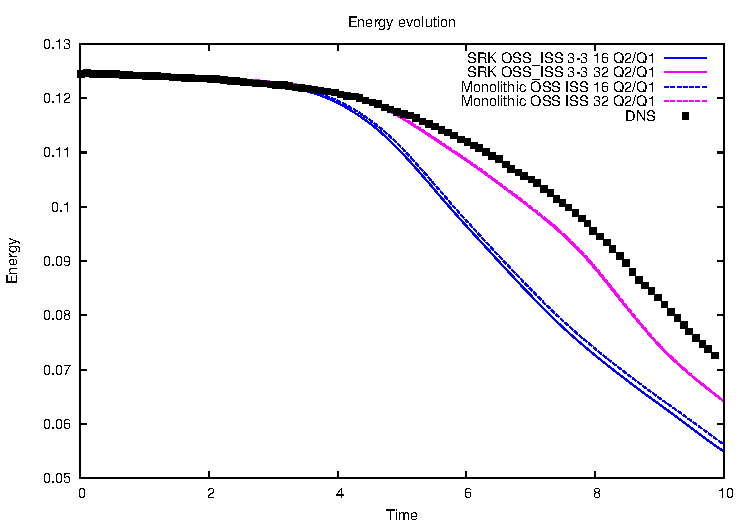
\includegraphics[width=0.49\textwidth]{Figures/Chapter7/TGV/srk_mono_ene}}
  \subfigure[Total energy dissipation rate]{\label{fig-TGV_SRK_mono_dis}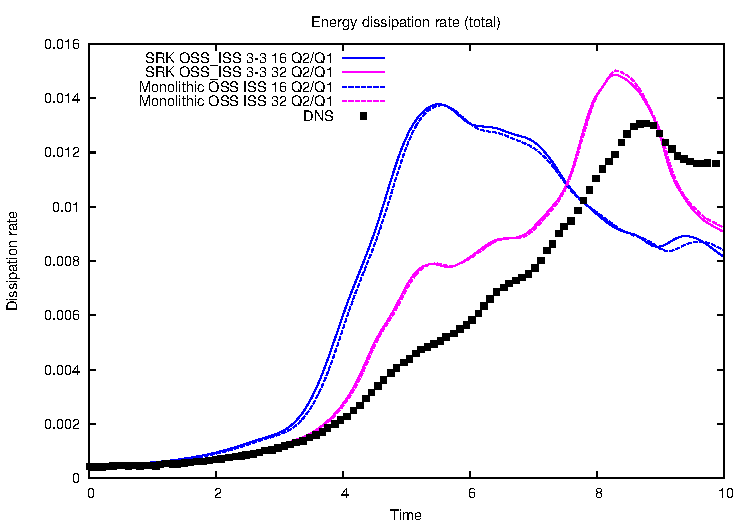
\includegraphics[width=0.49\textwidth]{Figures/Chapter7/TGV/srk_mono_tot}}
  \caption{Energy and Total energy dissipation rate evolution with $33^3$ velocity DOFs}
  \label{fig-TGV_SRK_mono_ene_dis}
\end{figure}

%It is important to point out that the main computational cost of an explicit SRK scheme is given by the solution of the pressure equations \Eq{C7_SRK_upeta_RK_p} and \Eq{C7_SRK_upeta_RK_p_n+1} that in practice are equivalent to solve a Darcy problem like \Eq{C7_SRK_upeta_RK_p_darcy}. The use of block preconditioning technique will lead to the solution of a mass matrix of the size of the velocity DOFs and a Laplacian matrix of the size of the pressure DOFs. Then, when using $Q_2/Q_1$ Finite Elements, the problem that will determine the computational cost will be the solution of the Laplacian matrix which is constructed by linear interpolation elements $Q_1$. Thus, when comparing the SRK method against a monolithic approach, it is fair to compare solutions of the same pressure DOFs instead of velocity DOFs.

\subsubsection{$h$-$p$ refinement and adaptive time-stepping technique}
\label{subsubsec-C7_TGV_hp_refinement}
In Fig \ref{fig-TGV_SRK_mono_ene_dis} we clearly see that refining the mesh, the results computed using the OSS-ISS method converge to the DNS. Moreover, it has been shown in \Chap{TBT_OSS} that a $ 32^3 $ $ Q_3/Q_2 $ elements mesh is fine enough to get very accurate results with the OSS-ISS method.

One of the main problems when using explicit or IMEX time integration schemes is the restriction on the CFL number. In the case of the IMEX version of the SRK scheme, the diffusive term is treated implicitly and no restriction has to be satisfied for the parabolic CFL, but the convective term is treated explicitly. Then, we have to restrict the time step size in order to satisfy the parabolic CFL condition, $ \mbox{CFL}_u=\delta tu/h<1 $. This restriction becomes more important when the mesh is refined, i. e. $ h $ is reduced.

An important goal of using SRK schemes is the possibility to easily implement an adaptive time stepping technique, see section \ref{subsec-C7_adaptive}. The important point of using this kind of techniques is that one can dynamicaly (and automaticaly) adapt the time step in order to satisfy both, the physical and numerical, requirements. The physical requirement on the time step size will be given by the change in the solution, while the numerical requirement will be given by the CFL condition.

In order to check the performance of the SRK method using adaptive time stepping, we solve the TGV problem with different mesh sizes and interpolations. Particularly, we use $ 16^3 $ and $ 32^3 $ elements mesh with $ Q_2/Q_1 $ and $ Q_3/Q_2 $ discretizations, depicted in Fig \ref{fig-TGV_SRK_refinement}.
\begin{figure}[h!]
  \centering
  \subfigure[Energy evolution]{\label{fig-TGV_SRK_ref_ene}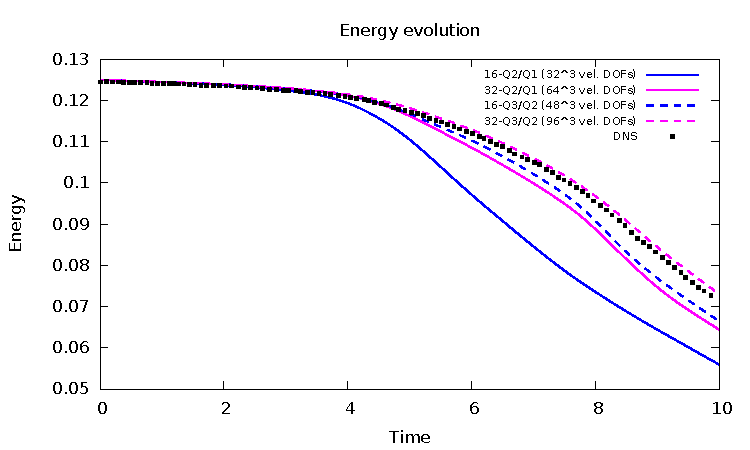
\includegraphics[width=0.49\textwidth]{Figures/Chapter7/TGV/refinement_ene}}
  \subfigure[Total energy dissipation rate]{\label{fig-TGV_SRK_ref_dis}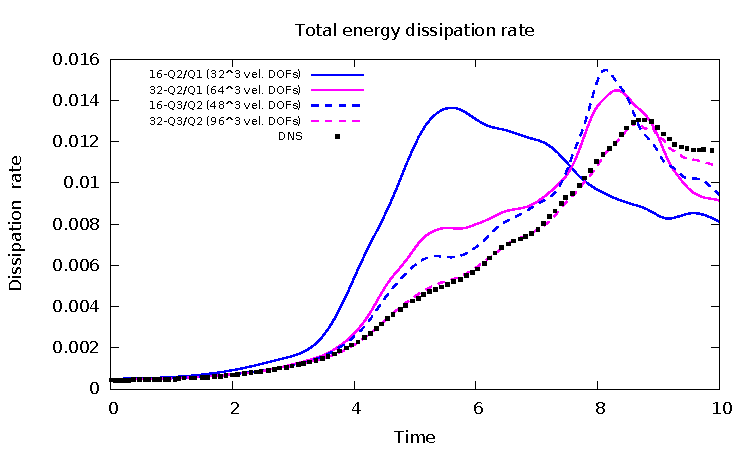
\includegraphics[width=0.49\textwidth]{Figures/Chapter7/TGV/refinement_dis}}
  \caption{Energy and total energy dissipation rate evolution refining the mesh}
  \label{fig-TGV_SRK_refinement}
\end{figure}
Looking at the kinetic energy evolution (\Fig{TGV_SRK_ref_ene}) and at the total energy dissipation rate (\Fig{TGV_SRK_ref_dis}), we can clearly see that when the mesh is refined the solution tends to the DNS result. It is important to highlight here the improvement of the results when higher order of approximation is used. We see that using $ Q_3/Q_2 $ elements we get better results than using $ Q_2/Q_1 $, even with less DOFs. This behaviour is observed comparing the $ 16^3 $ $ Q_3/Q_2 $ elements mesh, with $ 48^3 $ velocity DOFs, against the $ 32^3 $ $ Q_2/Q_1 $ elements discretization, which have $ 64^3 $ velocity DOFs. It is seen that the former mesh have better agreement with the DNS solution.

As stated above, the mesh refinement has a direct implication in the time step size when explicit or IMEX schemes are used. To determine the influence of this refinement using an adaptive time stepping technique, we show the time step evolution for the four cases considered in this subsection, see \Fig{TGV_SRK_tim}. The initial time step is $ \delta t_0=5\cdot10^{-2} $ for all cases. It is seen that the coarser mesh ($ 16^3 $ $ Q_2/Q_1 $ elements) allow a higher time step, which is constantly increased until the difference on the solution between to time steps is too high. It occurs around $ t=4.0 $, moment from which the time step size is adapted, remaining between $ 0.1 $ and $ 0.12 $. The $ 16^3 $ $ Q_3/Q_2 $ and the $ 32^3 $ $ Q_2/Q_1 $ show moreorless the same behaviour, with a first stage where the time step is increased until the CFL restriction is violated, point at which the time step is reduced. This pattern is repeated until the solution between two time steps is different enough to require a smaller time step to give more accurate solution. In what concerns the finest mesh, $ 32^3 $ $ Q_3/Q_2 $, the CFL restriction prevails over the physical phenomena restriction. Consequently, the time step increase-decrease pattern is followed during the whole simulation.
\begin{figure}[h!]
  \centering
  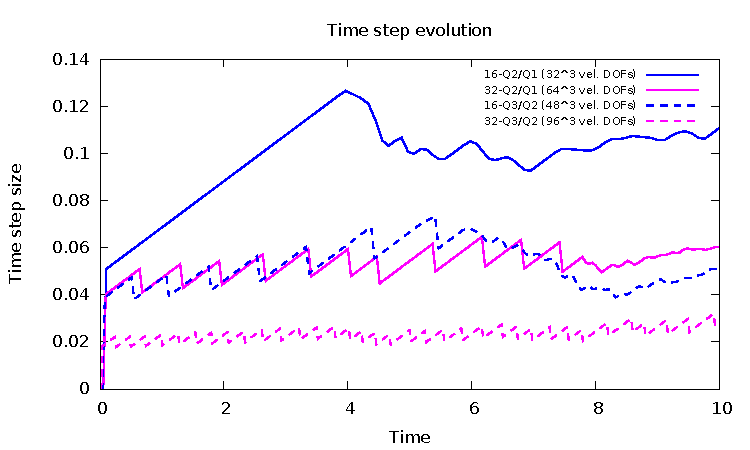
\includegraphics[width=0.6\textwidth]{Figures/Chapter7/TGV/refinement_dtime}
  \caption{Time step size evolution refining the mesh}
  \label{fig-TGV_SRK_tim}
\end{figure}

\subsubsection{Scalability analysis}
All the solutions have been computed with FEMPAR (Finite Element Multiphysics and massively PARallel) numerical software. FEMPAR is an open source in-house developed, parallel hybrid OpenMP/MPI, object-oriented (OO) framework which, among other features, provides the basic tools for the efficient parallel distributed-memory implementation  of substructuring domain decomposition solvers~\cite{badia_implementation_2013,badia_highly_2014}. Under this parallel framework, an important issue is the scalability of the algorithms when large scale problems are solved. This means that when refining the mesh, there is the need of having scalable solvers that do not increase the elapsed CPU time when the number of processors are increased. To check the suitability of the explicit SRK algorithm for large scale problems we perform a weak scalability test solving the TGV problem. 

Let us denote $ H $ the unidirectional size of the domain partition and $ L $ the unidirectional domain length. The TGV problem is solved in a domain of size $ L^3 $, with structured subdomain partitions of size $ H^3 $, and with a uniformly structured mesh composed of elements of size $ h^3 $. In a weak scalability test we keep the local meshes constant, that is to keep the number of elements per processor constant, which means that $ H/h= C $. In order to preserve the numerical properties, i. e. keep $ h $ constant, instead of reducing $ h $ we increase $ L $. Hence, as the reference problem is computed in a domain of size $ L_0=2\pi $, the scalabitilty analysis will be done in a domain of size $ L=\beta L_0 $, being $ \beta=\{1,2,3,4,5\} $. The reference partition size is $ H_0=L_0/4 $ and will be kept constant.

We compute the solution after one time step of size $\delta t=5\cdot10^{-2}$ with the IMEX version of the \textit{(1-2)} scheme (see Appendix \ref{appendix-butcher_tableaus}), using the $ Q_2/Q_1 $ element type, and reporting the number of solver iterations and the CPU time consumed by each system resolution. Different local mesh sizes are considered to see the effect of the local mesh size on the scalability of the solver. In particular, we will consider three cases: $ H/h=\{4,8,12\} $. The total amount of processors used to solve the problem will be $ (L/H)^3 = (4\beta)^3 $. The smallest mesh used to solve the problem in this analysis is a $ 16^3 $ $ Q_2/Q_1 $ elements mesh, while the biggest one is a $ 240^3 $ $ Q_2/Q_1 $ elements mesh, which give more than $ 680 $ million DOFs.

The following results are computed with a two-level BDDC solver, considering the corners, edges and faces of the subdomain partitions as part of the coarse system. We recall that the first step of a SRK \textit{(1-2)} scheme consist in six system resolutions that are specified in Algorithm \ref{alg-SRK_solvers}.
\begin{algorithm}
\caption{SRK system resolutions for one time step using the \textit{(1-2)} scheme}
\label{alg-SRK_solvers}
\begin{enumerate}
\item Solve initial pressure (equation \Eq{C7_SRK_upeta_RK_p}).
\item Solve second-stage momentum system (equations \Eq{C7_SRK_upeta_RK_u}-\Eq{C7_SRK_upeta_RK_eta}).
\item Solve second-stage pressure (equation \Eq{C7_SRK_upeta_RK_p}).
\item Solve velocity update (equation \Eq{C7_SRK_upeta_RK_u_n+1}).
\item Solve projection update (equation \Eq{C7_SRK_upeta_RK_eta_n+1}).
\item Solve pressure update (equation \Eq{C7_SRK_upeta_RK_p_n+1}).
\end{enumerate}
\end{algorithm}
Note that the first system solver is only needed at the first step, since after that $ p_1=p_n $.

\Fig{TGV_SRK_scal} depicts the solver iterations and the elapsed CPU time for the weak scalability analysis with the three different local mesh sizes. All the six system solvers are depicted in the solver iteration plots (\Fig{TGV_SRK_scal_iter_4}, \Fig{TGV_SRK_scal_iter_8} and \Fig{TGV_SRK_scal_iter_12}), while for the CPU time graphics (\Fig{TGV_SRK_scal_time_4}, \Fig{TGV_SRK_scal_time_8} and \Fig{TGV_SRK_scal_time_12}) the pressure system resolutions have been grouped and the building time has been added. The building time includes the time consumed to integrate all matrices and vectors and the time consumed computing the preconditioners.
\begin{figure}[p]
  \centering
  \subfigure[Iterations, $H/h=4$]{\label{fig-TGV_SRK_scal_iter_4}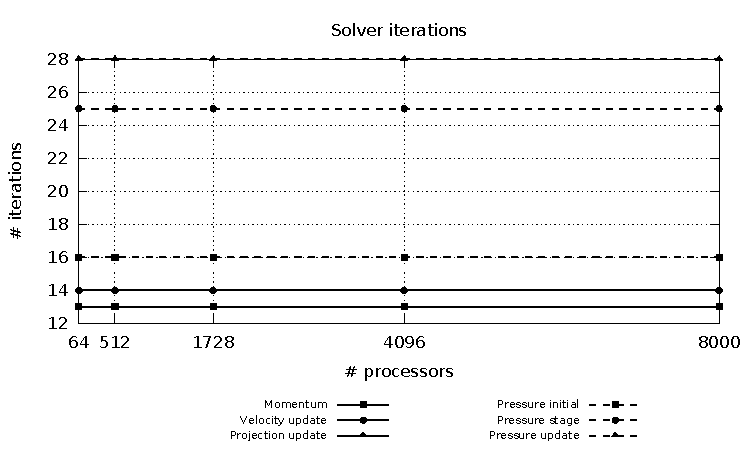
\includegraphics[width=0.49\textwidth]{Figures/Chapter7/TGV/iter_4_cef}}
  \subfigure[CPU time, $H/h=4$]{\label{fig-TGV_SRK_scal_time_4}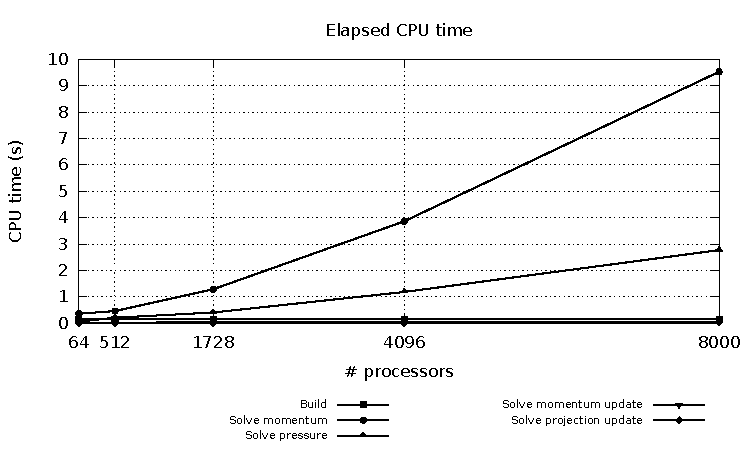
\includegraphics[width=0.49\textwidth]{Figures/Chapter7/TGV/time_4_cef}}\\
  \subfigure[Iterations, $H/h=8$]{\label{fig-TGV_SRK_scal_iter_8}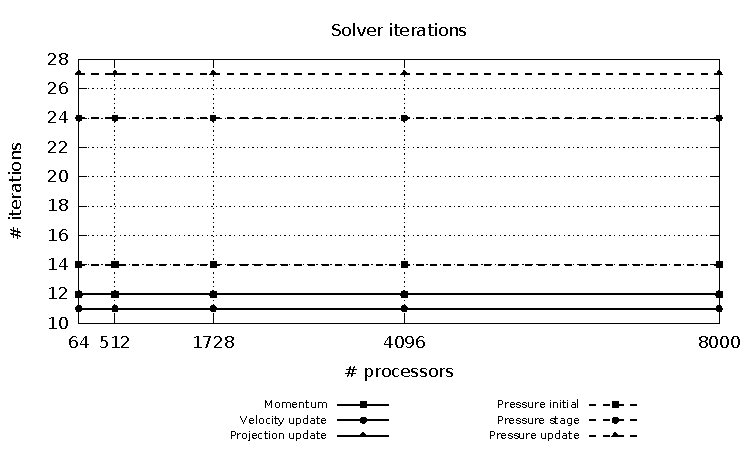
\includegraphics[width=0.49\textwidth]{Figures/Chapter7/TGV/iter_8_cef}}
  \subfigure[CPU time, $H/h=8$]{\label{fig-TGV_SRK_scal_time_8}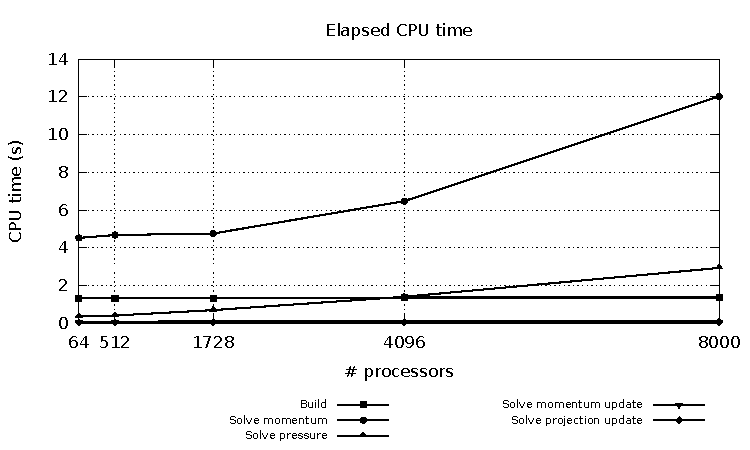
\includegraphics[width=0.49\textwidth]{Figures/Chapter7/TGV/time_8_cef}}\\
  \subfigure[Iterations, $H/h=12$]{\label{fig-TGV_SRK_scal_iter_12}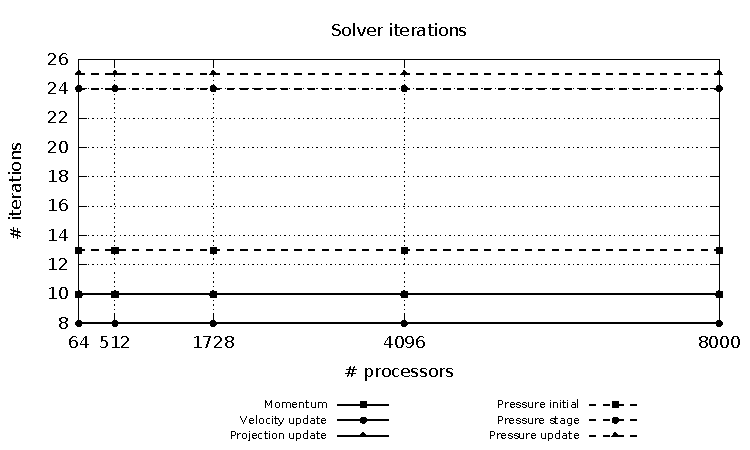
\includegraphics[width=0.49\textwidth]{Figures/Chapter7/TGV/iter_12_cef}}
  \subfigure[CPU time, $H/h=12$]{\label{fig-TGV_SRK_scal_time_12}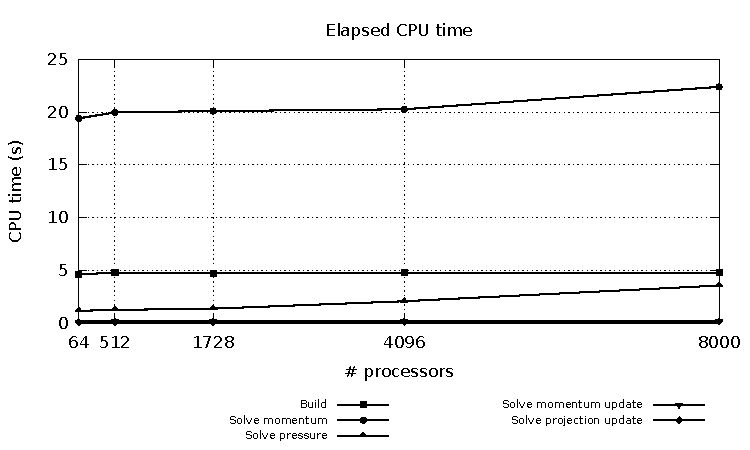
\includegraphics[width=0.49\textwidth]{Figures/Chapter7/TGV/time_12_cef}}\\
  \caption{Weak scalability test. Number of iterations and elapsed CPU time for solving one time step of the TGV problem with different local mesh sizes.}
  \label{fig-TGV_SRK_scal}
\end{figure}

Looking at the solver iterations, we see that the number of iterations for each system resolution is kept constant when the number of processors is increased, independently of the local mesh size. We notice that when the local mesh sizes increase, the number of iterations decrease a little for all systems. Another thing that we must point out looking at the solver iterations column in \Fig{TGV_SRK_scal} is that, as expected, the velocity update and the projection update give the same number of solver iterations. This is caused by the fact that both systems solve a mass matrix, with the only difference that the velocity update mass matrix is scaled by $ \frac{1}{\delta t} $. We also see that, in terms of solver iterations, the hardest system is the pressure computation (equations \Eq{C7_SRK_upeta_RK_p} and \Eq{C7_SRK_upeta_RK_p_n+1}). This behaviour is also expected, since the preconditioner of the schur complement ...

In what refers to the consumed CPU time, a first conclusion we can take looking at \Fig{TGV_SRK_scal_time_4}, \Fig{TGV_SRK_scal_time_8} and \Fig{TGV_SRK_scal_time_12} is that the most expensive resolution is the momentum system (equations \Eq{C7_SRK_upeta_RK_u}-\Eq{C7_SRK_upeta_RK_eta}). Although the number of solver iterations is smaller than the pressure computations, in terms of time consumed, the momentum equations resolution is much expensive, even counting together the three pressure solvers. This difference in the computational time required for the momentum equations versus the pressure ones, is due to the number of DOFs that are being solved. We have to take into account that both velocity and projection fields are computed with a second order polynomial, $ Q_2 $, while the pressure is first order, $ Q_1 $. Then, we not only have two vectorial fields versus a scalar field, but we have a second order interpolation versus a first order. Leaving aside the mass matrix blocks, the size of the system of equations to be solved in the velocity block of the momentum computation is $ \sim24 $ times larger than the one that arise for the pressure block of the Darcy computations, taking into account that the pressure system is solved using \Eq{C7_SRK_upeta_RK_p_darcy_weak}.

keeping with the discussion about the CPU time consumed shown in \Fig{TGV_SRK_scal}, we see that the computations of the momentum and pressure systems do not scale in terms of time. This performance has an easy explanation, which is given by the ratio between the fine and coarse system sizes. The coarse system size only depends on the number of processors (subdomains) used by the BDDC method. When corners, edges and faces of the subdomain are considered, the total amount of degrees of freedom of the coarse system is equivalent to a local mesh of $ Q_2 $ elements (without the interior node) with as many elements as subdomains. Consequently, for a $ H/h=4 $ local mesh, we can only expect to have weak scalability until $ 64 $ ($ 4^3 $) processors, for $ H/h=8 $ until $ 512 $ ($ 8^3 $) processors, and for $ H/h=12 $ until $ 1728 $ ($ 12^3 $) processors. In fact this is what we are seeing in \Fig{TGV_SRK_scal}, where, taking into account that the local meshes have the interior DOF inside each element, the results show the expected scalability performance.

In order to have even better results, one can reduce the size of the coarse system by considering only the corners and the edges of the subdomain. In \Fig{TGV_SRK_scal_ce} we depict the results obtained in this case, for a $ H/h=12 $ local mesh size. It is seen that when the subdomain faces are ignored, the number of solver iterations increase, see \Fig{TGV_SRK_scal_iter_12_ce}. Despite that, in the trade-off of having more solver iterations with smaller system of equations, ignoring the subdomain faces in the coarse system worth. As we can see in \Fig{TGV_SRK_scal_time_12_ce}, the momentum system is scalable up to 8.000 processors since the local problem is more expensive than the coarse one. We can not scale in time for the pressure solver because the local problem is much smaller than the coarse as we use $ Q_1 $ elements for the pressure field.
\begin{figure}[h!]
  \centering
  \subfigure[Iterations]{\label{fig-TGV_SRK_scal_iter_12_ce}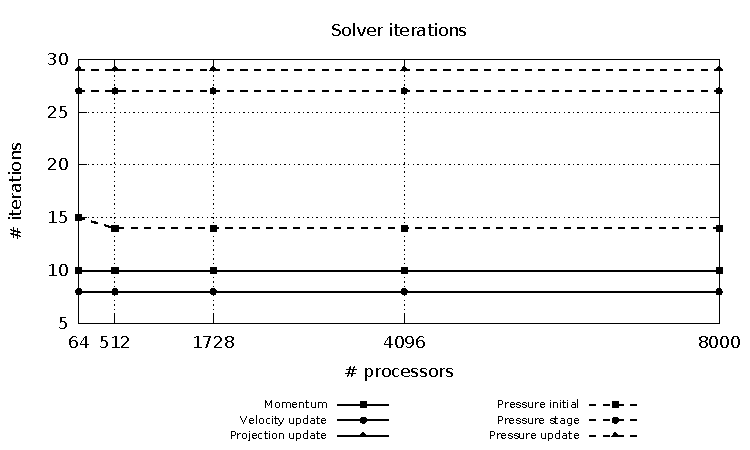
\includegraphics[width=0.49\textwidth]{Figures/Chapter7/TGV/iter_12_ce}}
  \subfigure[CPU time]{\label{fig-TGV_SRK_scal_time_12_ce}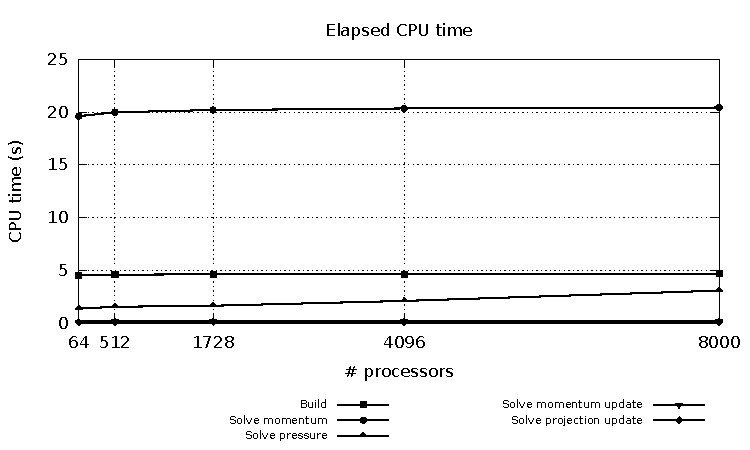
\includegraphics[width=0.49\textwidth]{Figures/Chapter7/TGV/time_12_ce}}\\
  \caption{Weak scalability test. Number of iterations and elapsed CPU time for solving one time step of the TGV problem with $ H/h=12 $ and only corners and edges at the coarse level.}
  \label{fig-TGV_SRK_scal_ce}
\end{figure}

Although that the weak scalability of the proposed method have been demonstrated up to 8000 processors, we could go further making use of a three-level method as it is defined in the multilevel implementation MLBDDC proposed in \cite{alberto_f._martin_santiago_badia_and_javier_principe_multilevel_????}.

\subsection{Turbulent channel flow at $Re_\tau=395$}
\label{subsec-C7_TCF}
In the previous section we have tested the suitability of the proposed VMS method using an IMEX SRK time integration scheme for the LES simulation of homogeneous turbulence. After that, we aim to show the performance of such methods for wall-bounded turbulent flows. In order to check the behaviour of the proposed approach, we solve the TCF test with a Reynolds number based on the wall velocity $ Re_\tau=395 $.

One of the main purposed of this test is to assess the accuracy of the solution when using the weak boundary conditions formulation given by the bilinear form described in \Eq{C7_bilinear_weak_by_components}. Then, the TCF test is suitable for this assessment.

\subsubsection{Setting}
The TCF problem is solved in a boxed domain of size $(2\pi\delta\times 2\delta\times 2/3\pi\delta)$. Where the $x$-direction is the flow direction, also called stream-wise direction, the $y$-direction is the wall-normal direction, and the $z$-direction is the span-wise direction. Homogeneous Dirichlet boundary conditions for the velocity DOFs are weakly imposed on wall-normal direction boundaries ($y=-\delta$ and $y=\delta$), while periodic boundary conditions are defined on the stream-wise and span-wise directions. We refer to Section \ref{subsubsec-C3_TCF} for a deeper description of this test.

We select the problem parameters according to the DNS computation performed by Moser et al in \cite{moser_direct_1999,kim_turbulence_1987} (MKM-DNS), so we can compare our results with the cited work. The bulk mean velocity and the half channel height are taken equal to one, $\bar{U}=1$ and $\delta=1$. The estimated Reynolds number based on the bulk mean velocity is known, $Re=\bar{U}2\delta/\nu\approx 13,750$ (see \cite{pope_turbulent_2000}). Therefore, one can obtain the value of the viscosity, $\nu=1.4545\cdot10^{-4}$, and from the Reynolds number based on the friction velocity, we can determine the friction velocity magnitude: $u_\tau=Re_\tau\nu/\delta=5.745\cdot10^{-2}$. Thus, the wall shear stress reads $\tau_w=u_\tau^2=3.3010\cdot10^{-3}$. A force equivalent to a pressure gradient is imposed to drive the movement of the flow in the stream-wise direction, $f_x=\tau_w/\delta$.

As we have done in Section \ref{subsec-C5_turb_channel}, an initial solution proposed in \cite{moin_numerical_1980} is used to reach the statistically steady state faster, which consists in a unidirectional velocity profile over which is added a fluctuation:
\begin{align}
\label{eq-C7_TCF_initial_sol}
&u_x = C\left(1-y^8\right)+\epsilon\frac{L_x}{2}\sin(\pi y)\cos\left(\frac{4\pi x}{L_x}\right)\sin\left(\frac{2\pi z}{L_z}\right),\\\nonumber
&u_y = -\epsilon(1+\cos(\pi y))\sin(\pi y)\sin\left(\frac{4\pi x}{L_x}\right)\sin\left(\frac{2\pi z}{L_z}\right),\\
&u_z = -\epsilon\frac{L_z}{2}\sin\left(\frac{4\pi x}{L_x}\right)\sin(\pi y)\cos\left(\frac{2\pi z}{L_z}\right).\nonumber
\end{align}
The constant $C$ is chosen in a such way that the field without fluctuations would have a bulk mean velocity $\bar{U}=1.0$. The fluctuation constant $\epsilon$ is $10\%$ of the bulk mean velocity.

To solve the problem we use two different meshes, composed by $ 16^3 $ $ Q_2/Q_1 $ and $ Q_3/Q_2 $ elements. As a weak imposition of the boundary conditions is considered, we use uniformly distributed elements along the wall-normal direction. The effect of considering uniform or stretched meshes in the wall-normal direction is assessed in \cite{bazilevs_weak_2007}, concluding that similar results are achieved when weak Dirichlet boundary conditions are used.

According to the results obtained in \Chap{TBT_OSS}, the algorithmic constants that appear in \Eq{C7_tau_m} and \Eq{C7_tau_c} are chosen as $ c_1=12.0 $ and $ c_2=8.0 $. The constant that appear in the weak boundary conditions formulation is set to $ C_b=32.0 $. We will analyze the effect of the constant $ c_c $ for the current problem setting as it plays an important role when using inf-sup stable elements.
%
\subsubsection{Effect of $ c_c $ in uniform meshes}
In Section \ref{subsec-C5_turb_channel} we have analyzed the effect of the constant $ c_c $ that appear in equation \Eq{C7_tau_c_alt} for the case in which we have strong imposition of the boundary conditions together with the use of stretched meshes that capture the boundary layer. In this section we aim to check the performance of the method when changing the $ c_c $ algorithmic parameter in uniform meshes and weak boundary conditions imposition. In this case, in order to avoid the influence of the weak imposition of the wall normal component, we restrict strongly the wall-normal velocity, e.g. $ \u\cdot\n=0 $ on $ \Gamma_D $.

In \Fig{TCF_ene_ktc} we show the energy evolution of the solution for different values of $ c_c $ from $ t=0.0 $ to $ t=100.0 $, and computed on a $ 16^3 $ $ Q_2/Q_1 $ mesh. It can be shown that for uniform meshes, high values of $ c_c $ makes the solution more energy conserving, so the energy is not dissipating properly. The value $ c_c=1.0 $ is the first case that reaches the statistically stable state, at $ t\sim280.0 $, with the lowest global energy. Then, in following sections we will use $ c_c=1.0 $.
\begin{figure}[h!]
  \centering
  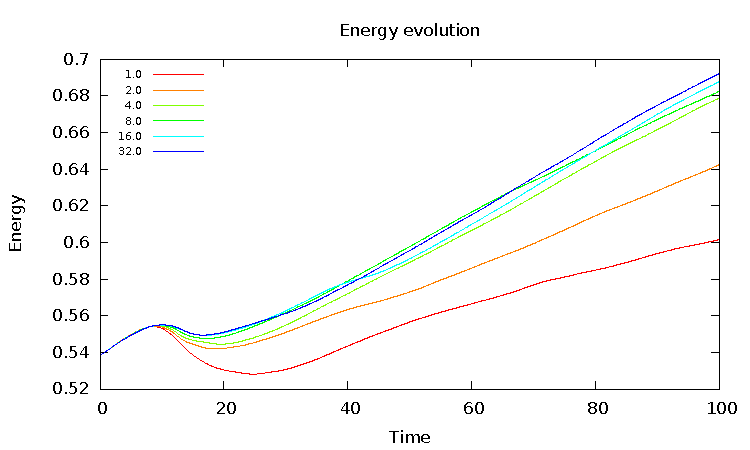
\includegraphics[width=0.6\textwidth]{Figures/Chapter7/TCF/ene_ktc}
  \caption{Energy evolution for the TCF test for different values of $ c_c $.}
  \label{fig-TCF_ene_ktc}
\end{figure}

\subsubsection{Influence of the wall-normal component}
\label{subsubsec-C7_TCF_wall_normal}
A significant difference on the approach followed for the weak enforcement of the Dirichlet boundary conditions considered in this work, with respect to the originally proposed in \cite{bazilevs_weak_2007}, is the treatment of the normal component. In \cite{bazilevs_weak_2007} a no-penetration condition is considered, which means that the normal component of the velocity is imposed strongly, $ \u\cdot\n=0 $ on $ \Gamma_D $. We propose to keep the weak boundary imposition even in the wall-normal direction. The main advantage of keeping the same approach for all components is revealed in curved boundaries. In that case, the different treatment of each component could lead to tedious code implementation.

As stated in section \ref{subsec-C7_weak_bcs}, we define two difference penalty parameters. One for the tangential component, based on the law of the wall, and another one for the wall-normal component, which is proportional to the original penalty parameter proposed in \cite{bazilevs_weak_2007-1}, $ \alpha_{b,n}:=\beta\frac{C_b\nu}{h_b} $. As it is obvious, when $ \beta\rightarrow\infty $ the solution at the wall becomes closer to the one obtained imposing strongly the normal component, but the penalty term may disturb the proper solution. 

In order to determine the best value for $ \beta $, we solve the TCF test from $ t=0.0 $ to $ t=100.0 $, with different values $ \beta=\{1.0,10,100,1000\} $ in a $ 16^3 $ $ Q_2/Q_1 $ elements mesh. The problem is solved using an IMEX SRK scheme with adaptive time adaptive technique.

In \Fig{TCF_ene_beta} we show the energy evolution for the different settings of $ \beta $. We clearly see that the choice of $ \beta $ has not a large implication on the results unless too low values of $ beta $ are used. For too low values of $ \beta $, the case of $ \beta=1.0 $, the solution starts dissipating too much energy at the early stages of the simulation. When increasing $ \beta $, the results tend to the ones obtained considering a strong imposition of the normal component, denoted by \textit{strong}. However, as it has been said before, the proposed method on uniform meshes is too little dissipative, so we will choose the value of $ \beta=10.0 $, which is a little bit more dissipative than greater values.
\begin{figure}[h!]
  \centering
  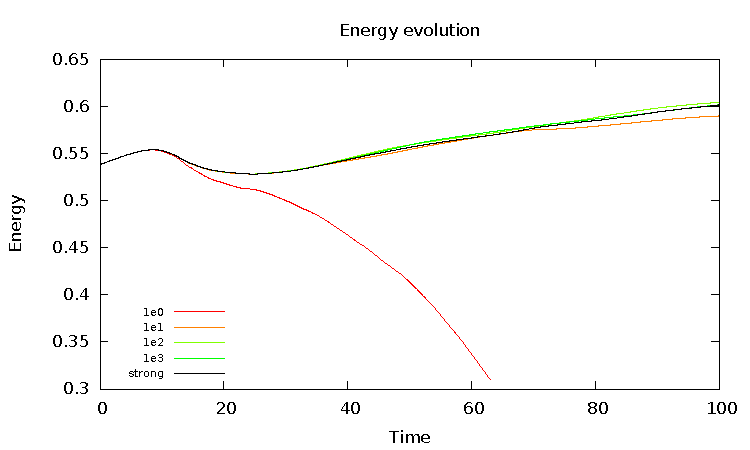
\includegraphics[width=0.6\textwidth]{Figures/Chapter7/TCF/ene_beta}
  \caption{Energy evolution for the TCF test for different values of $ \beta $.}
  \label{fig-TCF_ene_beta}
\end{figure}
%\begin{figure}[h!]
%  \centering
%  \subfigure[Energy evolution]{\label{fig-cha_ene}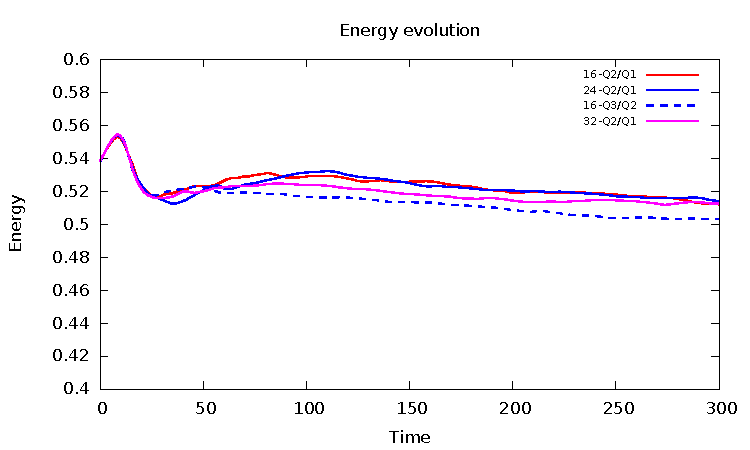
\includegraphics[width=0.49\textwidth]{Figures/TCF/ene}}
%  \subfigure[Time step size ($ \delta t $)]{\label{fig-cha_dtime}\includegraphics[width=0.49\textwidth]{Figures/TCF/dtime}}
%  \caption{Energy evolution and time step size for different values of $\beta$}
%  \label{fig-cha_ene_dtime}
%\end{figure}
%
%Note that with a fully implicit time integration scheme, the time step size required to solve properly the temporal scales for this problem is $ \delta t\sim0.03 $, see \cite{colomes_assessment}. Hence, the one given by the automatic adaptive time stepping for $ \beta=64 $ is $ \delta t\sim0.01 $, three times lower. This reduction on the time step size is compensated by the use of an explicit treatment of the convective term, with which we avoid the nonlinear iterations. For this particular case, with a $ 16^3 $ $ Q_2/Q_1 $ elements mesh, a time step resolution with an IMEX SRK scheme is around 6 times faster than a time step resolution with an implicit SRK scheme.
%
%The usage of IMEX SRK schemes only worths when uniform meshes are considered. Otherwise, when stretched meshes are employed to capture the boundary layer, the time step size restriction given by hyperbolic $ \mbox{CFL}_u $ make this schemes not affordable.
%
\subsubsection{Comparison between strong and week boundary conditions imposition}
Once analyzed the effect of the $ \beta $ parameter when Dirichlet boundary conditions are imposed weakly for the wall-normal component, let us check the performance of the approach followed in this work compared against a strong Dirichlet boundary conditions definition. We will compare with the results presented in \cite{colomes_mixed_2015}, where the TCF test was solved using strong Dirichlet boundary conditions in a stretched mesh. In Table \ref{tab-y_plus} we state the distance to the wall of the nearest velocity DOF for an stretched and a uniform mesh, with two different discretizations.
\begin{table}[h]
\caption{Distance to the wall of the nearest velocity DOF in wall units.}
\label{tab-y_plus}
\centering
\begin{tabular}{ccc}
\toprule
Mesh type&Discretization&$ y^+ $\\
\midrule
\midrule
\multirow{2}{*}{Stretched}&$ 16^3 $ $ Q_2/Q_1 $&$ 1.6 $\\
&$ 16^3 $ $ Q_3/Q_2 $&$ 1.0 $\\
\midrule
\multirow{2}{*}{Uniform}&$ 16^3 $ $ Q_2/Q_1 $&$ 24.7 $\\
&$ 16^3 $ $ Q_3/Q_2 $&$ 16.5 $\\
\bottomrule
\end{tabular}
\end{table}

The TCF test is solved from $ t=0.0 $ until the flow reach a statistically stable solution. In this case it is until $ t=300.0 $ for the $ 16^3 $ $ Q_2/Q_1 $ mesh and to $ t=240.0 $ for the $ 16^3 $ $ Q_3/Q_2 $ mesh. We store the statistics from the last $ 10.0 $ seconds, accumulating more than $ 1000 $ samples. The results are shown in \Fig{cha_vel}, where the mean stream-wise velocity is plotted (\Fig{cha_umean}) together with the velocity fluctuations in the stream-wise, wall-normal and span-wise directions (Figs. \ref{fig-cha_ufluc}, \ref{fig-cha_vfluc} and \ref{fig-cha_wfluc}, respectively).
\begin{figure}[h!]
	\centering	
	\subfigure[Mean stream-wise velocity]{\label{fig-cha_umean}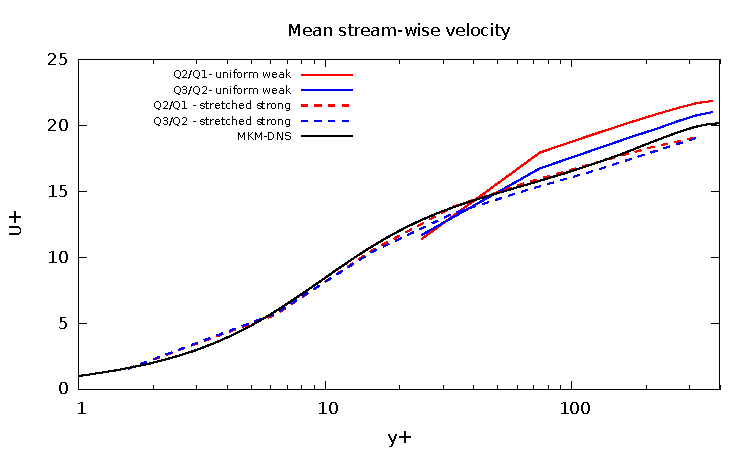
\includegraphics[width=0.49\textwidth]{Figures/Chapter7/TCF/umean}}
	\subfigure[Rms stream-wise velocity fluctuation]{\label{fig-cha_ufluc}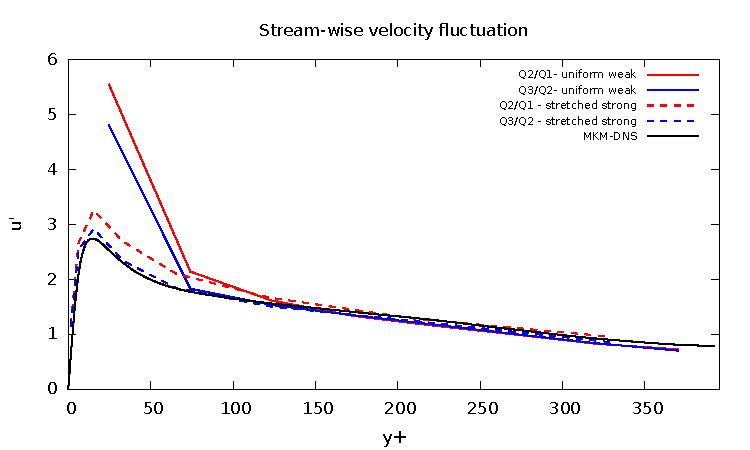
\includegraphics[width=0.49\textwidth]{Figures/Chapter7/TCF/ufluc}}\\   
  	\subfigure[Rms wall-normal velocity fluctuation]{\label{fig-cha_vfluc}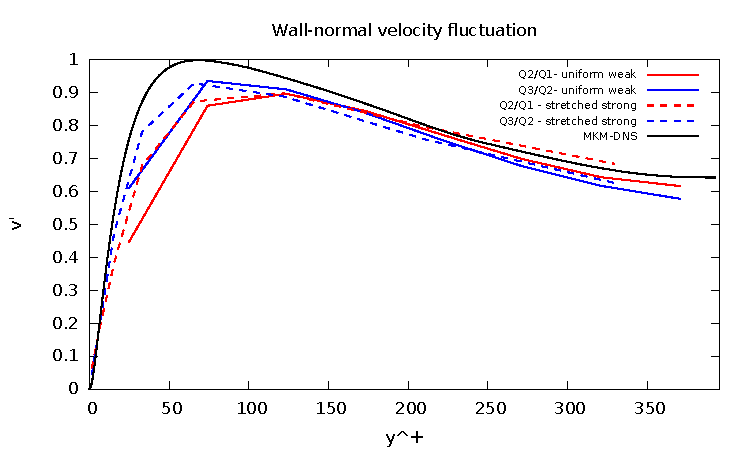
\includegraphics[width=0.49\textwidth]{Figures/Chapter7/TCF/vfluc}}
  	\subfigure[Rms span-wise velocity fluctuation]{\label{fig-cha_wfluc}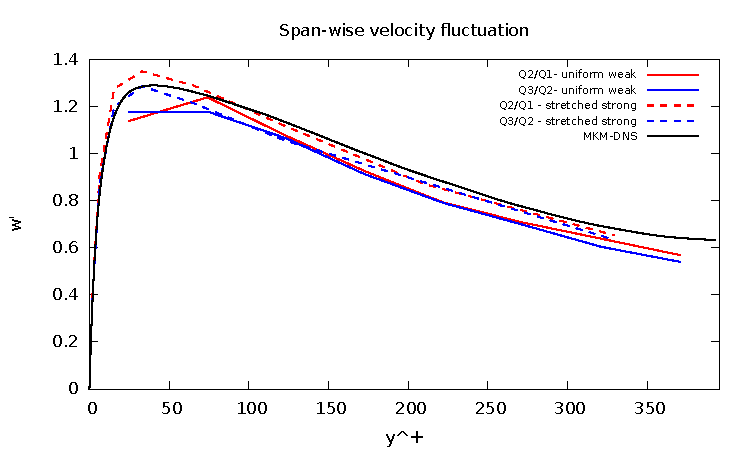
\includegraphics[width=0.49\textwidth]{Figures/Chapter7/TCF/wfluc}}
	\caption{Mean stream-wise velocity and rms velocity fluctuations for using different discretizations.}
	\label{fig-cha_vel}
\end{figure}

It is seen in \Fig{cha_umean} that the mean stream-wise velocity profile is a little bit far from the DNS results and also from the results obtained with strong boundary conditions in a stretched mesh. This behaviour is related to the energy evolution that we have shown in \Fig{TCF_ene_ktc}, where it is seen that the method does not dissipate the energy as it should.

%Particularly accurate are the results obtained with the $ 16^3 $ $ Q_3/Q_2 $ elements mesh, in which all points except the nearest to the wall are almost on top of the DNS curve, giving a better agreement to the DNS solution than the solution obtained with a stretched mesh.
%
Similar results are observed for the velocity fluctuations. Looking at \Fig{cha_ufluc}, where the stream-wise velocity fluctuation is depicted, we see that the nearest to the wall point is far to the DNS curve for the weak and uniform case, but we see that the remaining points fit to the desired results. As it is expected, an improvement in the solution is observed when higher order discretization is used. Same behaviour is observed for the wall-normal and span-wise velocity fluctuations, Figures \ref{fig-cha_vfluc} and \ref{fig-cha_wfluc}.

\section{Conclusions}
\label{sec-C7_conclusions}
In this chapter we have addressed the suitability of using SRK time integrations schemes for the LES of turbulent incompressible flows. A mixed FE formulation with convection stabilization through OSS method have been used for the spatial discretization of the Navier-Stokes equations, which, together with the SRK methods, conform a promising combination of spatial and temporal discretizations that are suitable for the simulation of turbulent incompressible flows. This particular combination have been denoted as \textit{Segregated Variational MultiScale}, SVMS, method.

The application of the SVMS method to the simulation of turbulent incompressible flows has been tested with the TGV test, showing that same results are achieved when considering a SRK time integration scheme instead of the traditional Crank-Nicolson scheme. The convergence to the DNS solution has also been demonstrated when a refinement both in $ h $ and $ p $ is considered, giving more accurate results the $ p $-refinement.

One of the advantages of using SRK schemes is the easy implementation of time adaptive techniques that allow the automatic time step adaptation to the numerical and physical requirements. This issue has also been addressed for the TGV test, where we have seen that the method is able to adapt to the numerical restriction given by the CFL conditions and to the physical requirements given by the change in the solution.

Another advantage of the SVMS methods is the possibility to use block preconditioning techniques that lead to the approximation of the inverse of Laplacian-type and elasticity-type matrices, which at his turn are suitable to be preconditioned with BDDC algorithms. The weak scalability of this approach for the resolution of one time step of the TGV test have been demonstrated up to 8000 cores. Furthermore, a three-level MLBDDC algorithm could be used to achieve weak scalability in a higher number of processors.

Moreover, aside from the TGV test, we have also checked the performance of SVMS method for the wall-bounded TCF test. In this case, we have also proposed the use of weak Dirichlet boundary conditions with the particularity of considering a wall-law based tangential traction and also a weak imposition of the wall-normal component.